\chapter{Exercise Solutions}
\begin{solution}[1.1]
Without any walls:
\begin{figure}[h]
	\centering
	\includegraphics[scale=0.9]{figures/solutions/ch1/S02D01.pdf}
\end{figure}

\begin{enumerate}
\item Case $\alpha > 0$:
\begin{figure}[h]
	\centering
	
\includegraphics[scale=0.9]{figures/solutions/ch1/Q01D01.pdf}
\end{figure}

\newpage 
\begin{enumerate}
\item Post impact velocity $ v(t_+) = -v(t_-)$ pre-impact velocity

\begin{figure}[h]
	\centering
	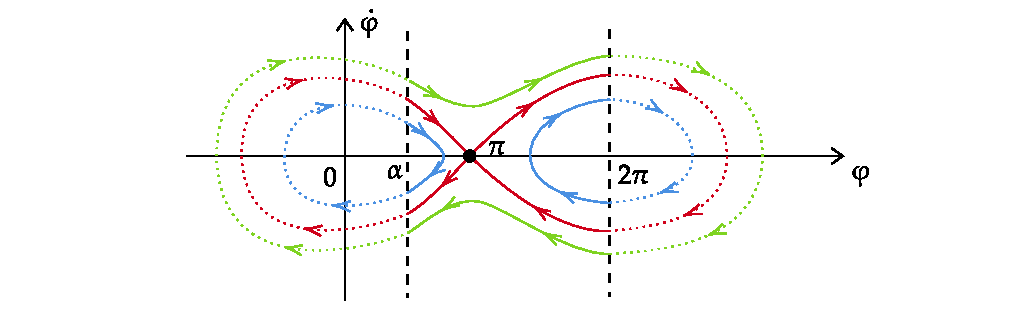
\includegraphics[scale=0.9]{figures/solutions/ch1/S02D02.pdf}
\end{figure}
The dashed lines represent the instance of impact.

Possible asymptotic behavior: depending on initial conditions $\varphi(0), \dot{\varphi}(0)$ 

\begin{itemize}
	\item {Bouncing against the inclined wall or the vertical wall;}
	\item {Bouncing back and forth between the two walls;}
	\item {Convergence to the upright position $\varphi = \pi, \dot{\varphi}=0$.}
\end{itemize}


\item Post impact velocity $ v(t_+) = -\frac{1}{2}v(t_-) $
\begin{figure}[h]
	\centering
	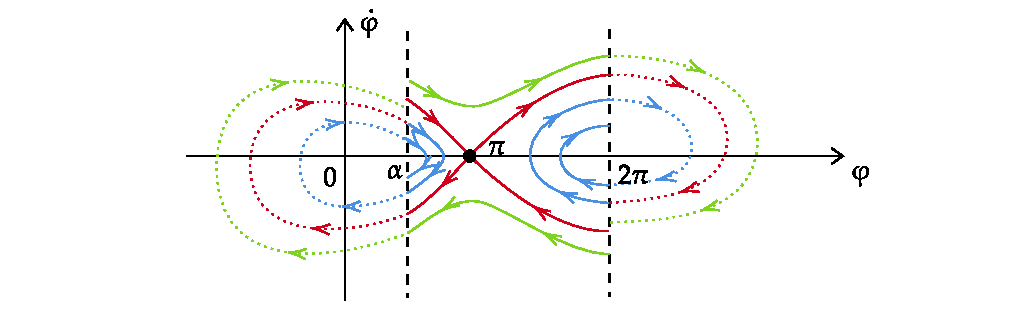
\includegraphics[scale=0.9]{figures/solutions/ch1/S02D03.pdf}
\end{figure}
Possible asymptotics:
\begin{itemize}
	\item Convergence to the upright position
	\item Lying against the inclined wall
	\item Lying against the vertical wall
\end{itemize}

\end{enumerate}
\newpage
\item Case $\alpha < 0$: Solution 1
\begin{figure}[h]
	\centering
	
\includegraphics[scale=0.9]{figures/solutions/ch1/S02D04.pdf}
\end{figure}

\begin{enumerate}
	\item $ v(t_+) = -v(t_-) $:

\begin{figure}[h]
	\centering
	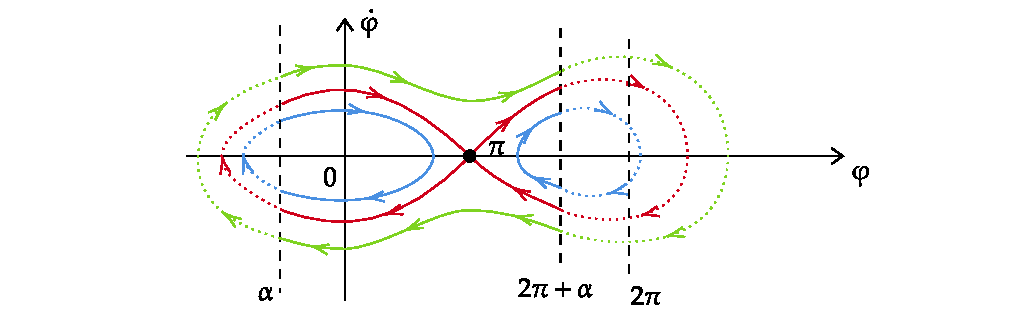
\includegraphics[scale=0.9]{figures/solutions/ch1/S02D05.pdf}
\end{figure}
Possible asymptotics:
\begin{itemize}
	\item Convergence to upright position
	\item Bouncing against either side of the wall
	\item Bouncing back an forth between the two sides of the wall
	\item Oscillating around the vertical position $\varphi = 0$
\end{itemize}


\item $ v(t_+) = -\frac{1}{2}v(t_-) $:
\begin{figure}[h]
	\centering
	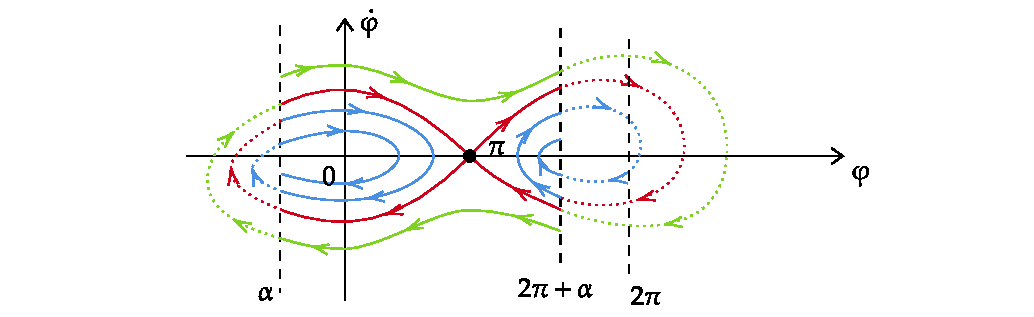
\includegraphics[scale=0.9]{figures/solutions/ch1/S02D06.pdf}
\end{figure}
Possible asymptotics:
\begin{itemize}
	\item Convergence to the upright position
	\item Oscillating around the vertical position $\varphi = 0$
	\item Lying on the back of the wall
\end{itemize}
\end{enumerate}
\newpage
\item Case $\alpha < 0$: Solution 2
\begin{figure}[h]
	\centering
	
\includegraphics[scale=0.9]{figures/solutions/ch1/S02D07.pdf}
\end{figure}

\begin{enumerate}
\item $ v(t_+) = -v(t_-) $:

\begin{figure}[h]
	\centering
	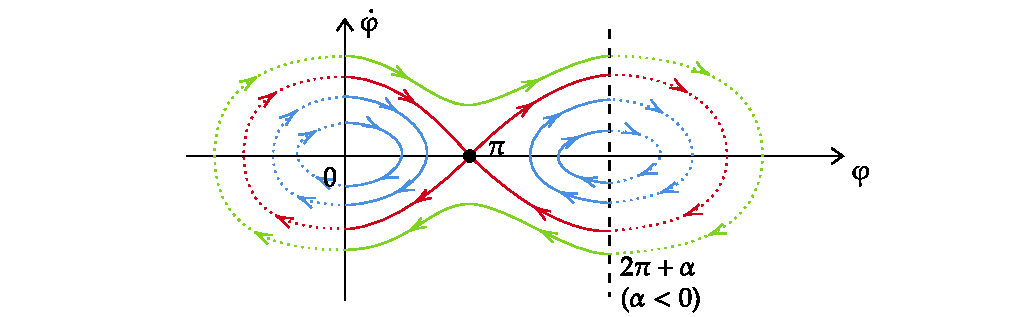
\includegraphics[scale=0.9]{figures/solutions/ch1/S02D08.pdf}
\end{figure}

\item Post impact velocity $ v(t_+) = -\frac{1}{2}v(t_-) $ pre-impact velocity
\begin{figure}[h]
	\centering
	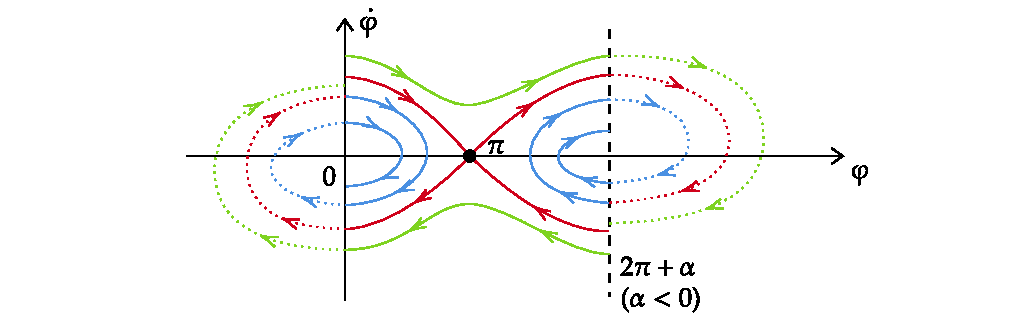
\includegraphics[scale=0.9]{figures/solutions/ch1/S02D09.pdf}
\end{figure}
Possible asymptotics:
\begin{itemize}
	\item Convergence to the upright position
	\item Lying against the inclined wall
	\item Lying against the vertical wall
\end{itemize}
\end{enumerate}

\end{enumerate}
\end{solution}


\begin{solution}[2.1] 
	\leavevmode
\begin{enumerate}
\item Define
\begin{align}\label{Sol1Ex1}
	h(t) = C + \int_{t_0}^t u(\tau)v(\tau)\,\text{d}\tau \\
	\Longrightarrow \dot{h}(t) = u(t)v(t) \leq^{(\ast)} v(t)h(t) 
\end{align}
From the definition of $h(t)$ and because $u,v>0$ we have $u(t) \leq h(t)$

\begin{align}\label{Sol1Ex2}
\Longrightarrow \frac{\dot{h}(t)}{h(t)} \leq v(t) \Longrightarrow \frac{d}{dt} \log \left[ h(t) \right] \leq v(t)
\end{align}
Integrate both sides of \eqref{Sol1Ex2} to get:
\begin{align}
	\log \left[ \frac{h(t)}{h(t_0)} \right] &\leq \int_{t_0}^t v(\tau)\,\text{d}\tau \\
	\Longrightarrow h(t) &\leq h(t_0) \exp\left( \int_{t_0}^t v(\tau)\,\text{d}\tau \right)
\end{align}
From \eqref{Sol1Ex1} we have $h(t_0)=C$; hence:
\begin{align}
	u(t) \leq h(t) \leq C \exp\left( \int_{t_0}^t v(\tau)\,\text{d}\tau \right)
\end{align}


\item The solutions $x(t,x_0)$ and $x(t,\tilde{x}_0)$ of the IVP satisfy the integral aligns
\begin{align}
	x(t,x_0) &= x_0 + \int_{t_0}^t f(x(s,x_0),s)\,\text{d}s \\
	x(t,\tilde{x}_0) &= x_0 + \int_{t_0}^t f(x(s,\tilde{x}_0),s)\,\text{d}s
\end{align}
Subtracting these two from each other and taking the absolute values we get
\begin{align}
	\left\vert x(t,x_0) - x(t,\tilde{x}_0) \right\vert = \left\vert x_0 - \tilde{x}_0 + \int_{t_0}^t \left[ f(x(s,x_0),s) - f(x(s,\tilde{x}_0),s) \right]\,\text{d}s \right\vert
\end{align}
Using triangular and Jensen's inequalities we get
\begin{align}\label{Sol1Ex3}
	\left\vert x(t,x_0) - x(t,\tilde{x}_0) \right\vert \leq \left\vert x_0 - \tilde{x}_0 \right\vert + \int_{t_0}^t \left\vert f(x(s,x_0),s) - f(x(s,\tilde{x}_0),s) \right\vert\,\text{d}s
\end{align}
By Lipschitz continuity of $f$ we have
\begin{align}
	\left\vert f(x(s,x_0),s) - f(x(s,\tilde{x}_0),s) \right\vert \leq L \left\vert x(t,x_0) - x(t,\tilde{x}_0) \right\vert
\end{align}
This together with \eqref{Sol1Ex3} gives
\begin{align}
	\left\vert x(t,x_0) - x(t,\tilde{x}_0) \right\vert \leq \left\vert x_0 - \tilde{x}_0 \right\vert + \int_{t_0}^t L \left\vert x(t,x_0) - x(t,\tilde{x}_0) \right\vert\,\text{d}s
\end{align}

Using Gronwall's inequality from Exercise 1.1 with
$u(t) = \vert x(t,x_0) - x(t,\tilde{x}_0) \vert$ , $C = \vert x_0 - \tilde{x}_0 \vert$ and $v(t) = L$ (constant), we get
\begin{align}
	\left\vert x(t,x_0) - x(t,\tilde{x}_0) \right\vert \leq \left\vert x_0 - \tilde{x}_0 \right\vert \exp \left( \int_{t_0}^t L\,\text{d}s \right) = \left\vert x_0 - \tilde{x}_0 \right\vert e^{L(t-t_0)}
\end{align}

\end{enumerate}
\end{solution}


\begin{solution}[2.2]
Pendulum equation:
\begin{align}
	\ddot{x} + k\dot{x} + \sin(x) = a \sin(t)
\end{align}
where $k \geq 0$ and $a \geq 0$

The first order system representation car be written as
\begin{align}
	z_1 &= x, \quad z_2 = \dot{x} \\
	\begin{bmatrix}
		\dot{z}_1 \\
		\dot{z}_2
	\end{bmatrix} &= \begin{bmatrix}
		z_2 \\
		a\sin(t) - kz_1 - \sin(z_1)
	\end{bmatrix}
\end{align}

Here is the Matlab code to produce the flowmap. 
\begin{verbatim}
%% Initialize script

close all
clear
clc

%% Grid of initial conditions

xs = linspace(-pi,pi,100);
ys = linspace(-pi,pi,100);
[X0, Y0] = meshgrid(xs,ys);

%% ODE simulation

t0 = 20;
tend = 0;

XF = zeros(size(X0));
YF = zeros(size(Y0));

for i = 1:size(X0,1)
    for j = 1:size(X0,2)
        x0 = X0(i,j);
        y0 = Y0(i,j);
        
        [t, z] = ode45(@odefun, [t0 tend], [x0,y0]);
        
        XF(i,j) = z(end,1);
        YF(i,j) = z(end,2);
    end
end

%% Deformation Gradient

[DFxx, DFxy] = gradient(XF, xs, ys);
[DFyx, DFyy] = gradient(YF, xs, ys);

%% Cauchy Green Strain Tensor Components

C11 = DFxx.^2 + DFyx.^2;
C12 = DFxx.*DFxy + DFyx.*DFyy;
C21 = C12;
C22 = DFxy.^2 + DFyy.^2;

%% Largest eigenvalue of Cauchy Green Strain Tensor

detC = C11.*C22 - C12.*C21;
traceC = C11 + C22;

lambda = real(traceC./2 + sqrt((traceC./2).^2 - detC));

%% PLot FTLE

FTLE = log(lambda)/(2*abs(tend-t0));

figure(1)
title('FTLE${}^{20}_0$', 'interpreter', 'latex')
surf(X0,Y0, FTLE, 'EdgeColor','none');
colorbar

axis tight
xlabel('$x$', 'interpreter','latex')
ylabel('$\dot{x}$', 'interpreter','latex')



%% Function to simulate

function [rhs] = odefun(t,X)
    a = 0.0; % or 0.5
    k = 0.0; % or 0.1
    
    x = X(1);
    xd = X(2);
    
    rhs = [xd;
            a*sin(t) - sin(x) - k*xd];
end
\end{verbatim}
\end{solution}


\begin{solution}[2.3]
\begin{align}
	\begin{dcases}
	\ddot{x} + \omega_0^2 x &= \varepsilon Mx^2, \quad 0 < \varepsilon \ll 1, \quad M>0, \quad \omega_0 \neq 0 \\
	x(0) &= a_0 \\
	\dot{x}(0) &= 0.
	\end{dcases}
\end{align}
\begin{itemize}
	\item Seek solutions of the form:
		\begin{align}
			x_\varepsilon(t) &= \varphi_0(t;\varepsilon) + \varepsilon\varphi_1(t;\varepsilon) + \mathcal{O}(\varepsilon^2) \\
			\varphi_i (t, \varepsilon) &= \varphi_i(t + T_\varepsilon; \varepsilon)
		\end{align}
	\item rewrite period as
		\begin{align}
			T_\varepsilon = \frac{2\pi}{\omega(\varepsilon)}, \quad \omega(\varepsilon) = \omega_0 + \varepsilon \omega_1 + \mathcal{O}(\varepsilon^2)
		\end{align}
	\item Rescale time: 
		\begin{align}
			\tau = \omega(\varepsilon)t \Longrightarrow \boxed{\frac{d}{d\tau} = \frac{1}{\omega(\varepsilon)}\frac{d}{dt}} \Longrightarrow \boxed{\left(\omega(\varepsilon)\right)^2x''+\omega_0^2 x = \varepsilon M x^2}
		\end{align}
	\item Plug in the new Ansatz into the rescaled equation
		\begin{align}
			[\omega_0^2 + 2\varepsilon \omega_0 \omega_1 + \mathcal{O}(\varepsilon^2)][\varphi_0'' + \varepsilon \varphi_1''+ \mathcal{O}(\varepsilon^2)] + \omega_0^2[\varphi_0 + \varepsilon \varphi_1+ \mathcal{O}(\varepsilon^2)] = \varepsilon M [\varphi_0^2 + \mathcal{O}(\varepsilon)]
		\end{align}
	\item Collect terms of equal power of $\varepsilon$
	
	$\mathcal{O}(1)$:
	\begin{align}
		\omega_0^2\varphi_0'' + \omega_0^2 \varphi_0 &= 0, \quad \varphi_0(0) = a_0, \quad \dot{\varphi}_0(0)=0 \\
		\Longrightarrow \varphi_0 &= a_0 \cos(\tau)
	\end{align}
	$\mathcal{O}(2)$:
	\begin{align}
		\omega_0^2\varphi_1'' + \omega_0^2 \varphi_1 &= M \varphi_0^2 - 2\omega_0\omega_1\varphi_0'' = Ma_0^2 \cos^2(\tau) + 2a_0\omega_0\omega_1 \cos(\tau) \\
		&= M \frac{a_0^2}{2}[1 + \cos(2\tau)] + \underbrace{2a_0\omega_0\omega_1\cos(\tau)}_{\text{resonance}}
	\end{align}
	Select $\omega_1 = 0$ to eliminate resonance terms and obtain periodic solution.
	
	Solve for $\varphi_1$:
	\begin{align} \label{S02E011}
		\varphi_1'' + \varphi_1 = \frac{Ma_0^2}{2\omega_0^2}[1 + \cos(2\tau)], \quad \varphi_1(0)=0, \quad \dot{\varphi}_1(0)=0
	\end{align}
	\item Pick solution Ansatz:
	\begin{align}
		\varphi_1(\tau) = A\cos(\tau) + B\sin(\tau) + C\cos(2\tau) + D\sin(2\tau) + E
	\end{align}
	\item Substituting in \eqref{S02E011}:
	\begin{align}
		&-A\cos(\tau) - B\sin(\tau) - 4C\cos(2\tau) - 4D\sin(2\tau) + A\cos(\tau) + B\sin(\tau) \\
		&\qquad+ C\cos(2\tau) + D\sin(2\tau) + E 
		= \frac{Ma_0^2}{2\omega_0^2}\cos(2\tau) + \frac{Ma_0^2}{2\omega_0^2}
	\end{align}
	\item Comparing coefficients:
	\begin{align}
		\Longrightarrow E = \frac{Ma_0^2}{2\omega_0^2}, \quad C = -\frac{Ma_0^2}{6\omega_0^2},\quad D=0
	\end{align}
	\begin{align}
		\varphi_1(0)=0 &\Longrightarrow A+C+E=0 \Longrightarrow A = -\frac{Ma_0^2}{3\omega_0^2} \\
		\varphi_1'(0)=0 &\Longrightarrow B+2D=0 \Longrightarrow B=0
	\end{align}
	\begin{align}
		\Longrightarrow \boxed{\varphi_1(\tau) = -\frac{Ma_0^2}{3\omega_0^2}\cos(\tau) - \frac{Ma_0^2}{6\omega_0^2}\cos(2\tau) + \frac{Ma_0^2}{2\omega_0^2}}
	\end{align}
	\item In original time:
	\begin{align}
		x_\varepsilon(t) = a_0\cos(\omega t) + \varepsilon \frac{Ma_0^2}{\omega_0^2} \left[ -\frac{1}{3}\cos(\omega t) - \frac{1}{6}\cos(2\omega t) + \frac{1}{2} \right] + \mathcal{O}(\varepsilon^2)
	\end{align}
	where
	\begin{align}
		\omega = \omega_0 + \mathcal{O}(\varepsilon^2)
	\end{align}
\end{itemize}
\end{solution}


\begin{solution}[2.4]
	\leavevmode
\begin{enumerate}
\item Seek solutions of the form:
\begin{align}
	x_\varepsilon(t)=\varphi_0(t)+ \varepsilon\varphi_1(t) + \mathcal{O}(\varepsilon^2)
\end{align}
Substituting this solution in the ODE $\ddot{x} + \varepsilon(x^2-1)\dot{x} + x = F\cos(\omega t)$ we get:
\begin{align}
	\ddot{\varphi}_0 + \varphi_0 + \varepsilon(\ddot{\varphi}_1 + \varphi_1 + \varphi_0^2\dot{\varphi}_0 - \dot{\varphi}_0) + \mathcal{O}(\varepsilon^2) = F\cos(\omega t)
\end{align}
\begin{align}
	\Longrightarrow \mathcal{O}(1) &: \ddot{\varphi}_0 + \varphi_0 = F\cos(\omega t) \label{S02E021} \\
	\Longrightarrow \mathcal{O}(2) &: \ddot{\varphi}_1 + \varphi_1 = \dot{\varphi}_0(1-\varphi_0^2) \label{S02E022}
\end{align}
Since we seek solutions with period $\frac{2\pi}{\omega}$ for any $0\leq \varepsilon \ll 1$, the period of each $\varphi_i$ must be $\frac{2\pi}{\omega}$.
Because the initial condition for the system was not specified we will use those to enforce the periodicity condition. That is, we assume that the initial conditions also depend on $\varepsilon$.
\begin{align}
x_\varepsilon(0) &= a + b\varepsilon + O(\varepsilon^2) \\
\dot{x}_\varepsilon(0) &= c + d\varepsilon + O(\varepsilon^2) \\
\end{align}

The solution that is $O(\varepsilon)$ accurate, can be obtained as a solution to equation \eqref{S02E021}. We take the following trial function 

\begin{align}
	\varphi_0(t) = A\sin(t) + B\cos(t) + C \cos(\omega t). \label{S02E023}
\end{align}

The constant $C$ can be determined by substituting into \ref{S02E021} as

$$
-C\omega^2 \cos(\omega t) + C\cos(\omega t) = F \cos(\omega t).
$$

Since this has to hold for all $t$, the coefficients of $\cos (\omega t)$ must balance. This leads to $C = F/(1-\omega^2)$. Therefore, the solution $\varphi_0(t)$ reads as 
\begin{align}
	\varphi_0(t) = A\sin(t) + B\cos(t) + \frac{F\cos(\omega t)}{1-\omega^2} \label{S02E023_2}.
\end{align}
To have a period  $\frac{2\pi}{\omega}$, we must select $A=B=0$. 
This condition can be enforced by choosing appropriate initial conditions for the ODE \eqref{S02E021}:
\begin{align}\label{S02E024}
	A=B=0 \Longrightarrow a = C = \frac{F}{1-\omega^2} \quad d =0. 
\end{align}
\begin{align}
\label{phi0}
\boxed{\varphi_0(t) = \frac{F\cos(\omega t)}{1-\omega^2}, \quad \varphi_0(0) = \frac{F}{1-\omega^2}, \quad \dot{\varphi}_0(0)=0}
\end{align}
\begin{align}
	x_\varepsilon(t) = \varphi_0(t) + \underbrace{\mathcal{O}(\varepsilon)}_\text{error term}
\end{align}

\subsection*{{\em Bonus: $O(\varepsilon^2)$ accurate calculation}}
We can proceed by solving the $O(\varepsilon)$ equation \eqref{S02E022}. With the solution \eqref{phi0} the forcing term on the right-hand side can be written as
\begin{align}
 \dot{\varphi}_0(1-\varphi_0^2) &= -C\omega \sin (\omega t)\left(1 - C^2 \cos^2 (\omega t)\right) \\
 & = -C\omega \sin(\omega t)\left(1 - C^2 + C^2\sin^2 (\omega t)\right)  \\
 & = -C\omega \sin(\omega t)(1 - C^2) - C^3\omega \sin^3 (\omega t) \\
 & = -C\omega(1-C^2) \sin(\omega t) - C^3 \omega \frac{3 \sin (\omega t) - \sin (3\omega t)}{4} \\
 & = C\omega\left(\frac{C^2}{4}-1\right)\sin (\omega t) + \frac{C^3 \omega }{4}\sin (3\omega t).
\end{align}

Equation \eqref{S02E022} now takes the form 

\begin{align}
\ddot{\varphi}_1 + \varphi_1 = C\omega\left(\frac{C^2}{4}-1\right)\sin (\omega t) + \frac{C^3 \omega }{4}\sin (3\omega t) ; \quad \varphi_1(0)=b \quad \dot{\varphi}_1(0)=d.
\end{align}

The appropriate trial functions is
\begin{align}
\varphi_1(t) = D \cos t + E \sin t + G \sin (\omega t) + H\sin(3 \omega t).
\end{align}
Upon substitution we find the following equation

$$
-G \omega^2 \sin (\omega t) - 9H\omega^2 \sin(3 \omega t) + G \sin (\omega t) + H\sin(3 \omega t) =  C\omega\left(\frac{C^2}{4}-1\right)\sin (\omega t) + \frac{C^3 \omega }{4}\sin (3\omega t) . 
$$
Balancing the coefficients of $\sin (\omega t)$ and $\sin (3\omega t)$ we end up with

\begin{align}
G &= \frac{C\omega }{(1-\omega^2)}\left(\frac{C^2}{4}-1\right)  \\
H &=\frac{C^3 \omega}{4(1-9\omega^2)}. 
\end{align}

To enforce periodicity with period $T = \frac{2\pi}{\omega}$  to order $\varepsilon$ we must have $D=E=0$. This can be achieved by choosing the initial conditions of the $\varphi_1$ equation appropriately. This means we must have

\begin{align}
\label{ic2}
\varphi_1(0) &= \boxed{b = 0 }\\
\dot{\varphi}_1(0) &= \boxed{G\omega + 3H \omega = d} .
\end{align}
Combining the solution $\varphi_1(t)$ with \eqref{phi0} we finally obtain, that the $T$-periodic solution is given by
\begin{align}
\label{phi1}
x_\varepsilon(t) &= \frac{F}{1-\omega^2}\cos (\omega t) + \varepsilon \frac{ F\omega}{(1-\omega^2)^2}\left(\frac{F^2}{4(1-\omega^2)^2}-1\right) \sin (\omega t) \\
& + \varepsilon \frac{F^3 \omega}{4(1-\omega^2)^3(1-9\omega^2)} \sin (3\omega t) \\
x_\varepsilon(0) & = \frac{F}{1-\omega^2} + O(\varepsilon^2) \\
\dot{x}_\varepsilon(0)  &=\varepsilon \left[\frac{F \omega^2}{(1-\omega^2)^2}\left( \frac{F^2}{4(1-\omega^2)^2}-1\right) + 3 \frac{F^3 \omega^2 }{4(1-\omega^2)^3(1-9\omega^2)}\right] + O(\varepsilon^2)
\end{align}

\item We solve the ODE numerically to obtain a solution $x(t)$ and compare this solution to the perturbed approximation $x_\varepsilon(t)$ given by \eqref{phi0} up to $O(\varepsilon)$.

The initial conditions for the ODE are chosen such that $x(0) = x_\varepsilon(0)$ and $\dot{x}(0) = \dot{x}_\varepsilon(0)$.

Therefore, $x(0)=\varphi_0(0), \quad \dot{x}(0) = \dot{\varphi}_0(0)$ where $\varphi_0(0)$ and $\dot{\varphi}_0(0)$ are given in \eqref{S02E024}.

Equivalent first order system of differential equations:
\begin{align}
\label{ode}
	z_1 = x, \quad z_2 = \dot{x}, \quad \begin{bmatrix}
		\dot{z}_1 \\
		\dot{z}_2
	\end{bmatrix} = \begin{bmatrix}
		z_2 \\
		F\cos(\omega t) - \varepsilon(z_1^2 - 1)z_2 - z_1
	\end{bmatrix}
\end{align}
\begin{figure}[h]
	\centering
	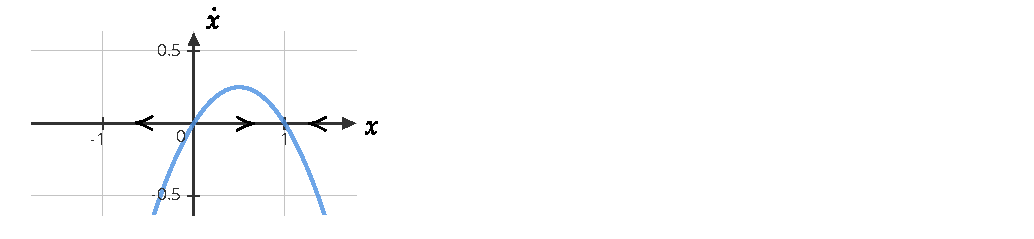
\includegraphics[scale=2]{figures/solutions/ch2/Q02D01.pdf}
\end{figure}

\item We now solve the same ODE \eqref{ode} numerically to obtain a solution $x(t)$ started from the $O(\varepsilon^2)$ accurate initial conditions given by \eqref{ic2} and compare this solution to refined perturbed approximation $x_\varepsilon(t)$ given by \eqref{phi1} up to $O(\varepsilon^2)$.

\begin{figure}[h]
	\centering
	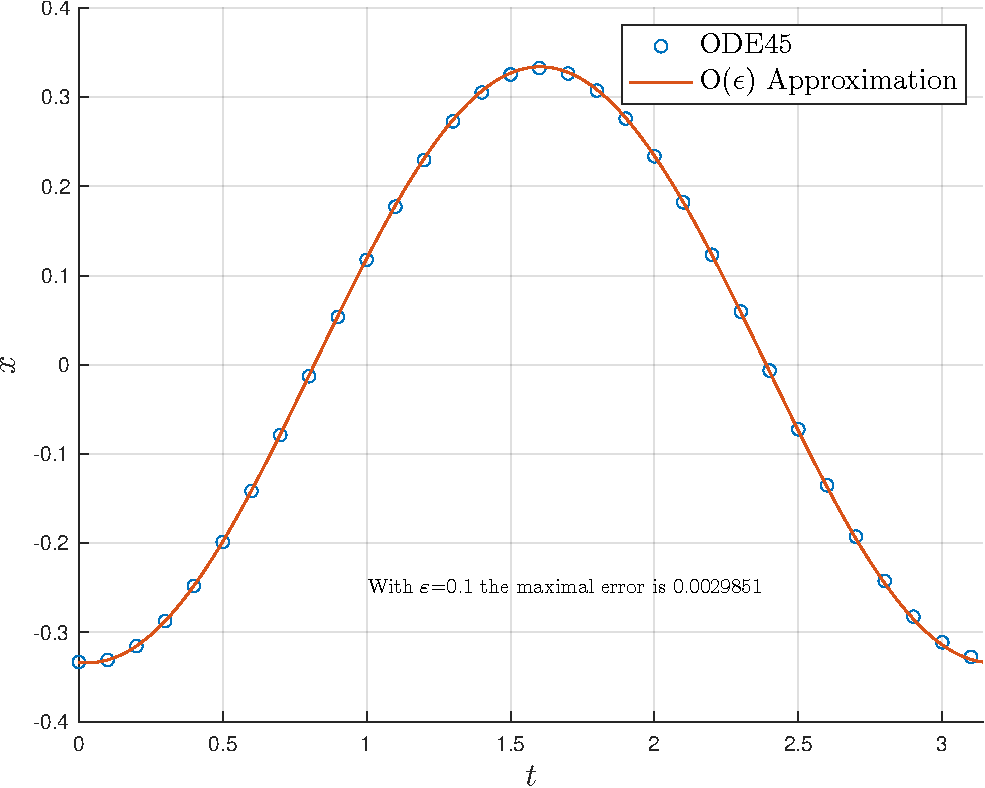
\includegraphics[scale=0.6]{figures/solutions/ch2/Q02D01_b.pdf}
\end{figure}

\end{enumerate}
\end{solution}


\begin{solution}[3.1]
	\leavevmode
\begin{enumerate}
\item Let $x_k$ be near the fixed point $P$ and define $y_k = x_k - P$. Then
\begin{align}
	x_{k+1} = f(x_k) = f(P + y_k) &= f(P) + Df(P)y_k + \mathcal{O}(||y_k||^2) \\
	&= P + Df(P)y_k + \mathcal{O}(||y_k||^2)
\end{align}
\begin{align}
	\Longrightarrow y_{k+1} = x_{k+1} - P = Df(P)y_k + \mathcal{O}(||y_k||^2)
\end{align}
Now for $||y_k||$ small enough the linear approximation of the map $x_{k+1} = f(x_k)$ is $y_{k+1} = Ay_k$ with $A = Df(P)$.


\item Take any $y_0 \in \mathbb{R}^n$. Since $s_1,\ldots ,s_n \in \mathbb{C}^n$ are linearly independent there are constants $c_1,\ldots ,c_n \in \mathbb{C}$ such that $y_0 = c_1s_1+\ldots+c_ns_n$.

Now define
\begin{align}
	y_1 = Ay_0 &= c_1As_1 + \cdots + c_nAs_n \\
	&= c_1\lambda s_1 + \cdots + c_n\lambda s_n \\
	&= c_1\varphi_1(1) + \cdots + c_n \varphi_n(1)
\end{align}
Similarly, for any $k \geq 1$,
\begin{align}
	y_k = Ay_{k-1} &= c_1 \lambda_1^{k-1}As_1 + \cdots + c_n \lambda_n^{k-1}As_n  \\
	&= c_1\varphi_1(k) + \cdots + c_n \varphi_n(k)
\end{align}
It's easy to check that $y_{k+1} = Ay_k$ for any $k \geq 0$. Since $y_0 \in \mathbb{R}^n$ was arbitrary, $c_1\varphi_1(k)+c_2\varphi_2(k) + \cdots + c_n\varphi_n(k)$ is a general solution of $y_{k+1} = Ay_k$.


\item We claim that the necessary and sufficient condition for asymptotic stability of the origin is $|\lambda_i|<1$ for $i=1,2,\ldots , n$

\underline{Sufficient}: From (c) any solution of $y_{k+1} = Ay_k$ can be written as:
\begin{align}
	y_{k+1} = \sum_{i=1}^n c_i \lambda_i^k s_i
\end{align}
Without loss of generality, we assume that the eigenvectors $s_i$ are normalized, i.e., $||s_i|| = 1 \,\forall i\in\{1,2,\ldots,n\}$. Then
\begin{align}
	||y_{k+1}|| \leq \sum_{i=1}^n |c_i||\lambda_i|^k ||s_i|| = \sum_{i=1}^n |c_i||\lambda_i|^k
\end{align}
But since $|\lambda_i|<1$, we have $\displaystyle \lim_{k \rightarrow \infty} |\lambda_i|^k = 0$. Which implies
\begin{align}
	\lim_{k \rightarrow \infty} \sum_{i=1}^n |c_i||\lambda_i|^k = 0
\end{align}
Hence, 
\begin{equation}\label{E0401}
	\lim_{k \rightarrow \infty} ||y_{k+1}||=0
\end{equation}
Also note that since $|\lambda_i|<1 \,\forall i\in \{1,\ldots,n\}$, the matrix norm $||A||<1$.

Hence $||y_{k+1}|| = ||Ay_k|| < ||y_k||. \Longrightarrow y=0$ is also stable. This together with (\ref{E0401}) implies asymptotic stability of the fixed point $y=0$.

\underline{Necessity}: Assume there is $i_0\in\{1,2,\ldots, n\}$ such that $|\lambda_{i_0}| \geq 1$.

It is enough to show that there exists $y_0 {\in\mathbb{R}^n}$ such that $\lim_{k \rightarrow \infty} ||A^ky_0|| \neq 0$.

This is due to the fact that $y_k = A^ky_0$ and that one can rescale $y_0$ as $ry_0$ for $0<r \ll 1$ small enough such that $||ry_0||<\delta, \,\forall \delta > 0$.

To show that such $y_0 \in \mathbb{R}^n$ exists, note that $||A^ks_{i_0}|| = ||\lambda_{i_0}^ks_{i_0}|| = |\lambda_{i_0}|^k \geq 1 \,\forall k \geq 0$.
\begin{remark}[]
	This is, however, not enough since $s_{i_0}\in\mathbb{C}^n$ while we need a vector in $\mathbb{R}^n$.
\end{remark}

To complete the proof, note that $s_{i_0}=\xi + i\eta$ with $\xi, \eta \in \mathbb{R}^n$.
\begin{align}
	\Longrightarrow 1 \leq ||A^ks_{i_0}||^2 = ||A^k\xi + i A^k\eta ||^2 = ||A^k\xi||^2 + ||A^k\eta||^2.
\end{align}
Therefore, either $||A^k\xi|| \geq \frac{1}{\sqrt{2}}$ or $||A^k\eta|| \geq \frac{1}{\sqrt{2}}$.

Without loss of generality assume $||A^k\xi|| \geq \frac{1}{\sqrt{2}}$. Now let $y_0 = \xi$ to get
\begin{align}
	\underbrace{||y_k|| = ||A^ky_0|| \geq \frac{1}{\sqrt{2}}}_{\text{true for every }k\geq 0} \Longrightarrow \lim_{k \rightarrow \infty} ||y_k|| \neq 0.
\end{align}
\end{enumerate}
\end{solution}

\begin{solution}[3.2]
	\leavevmode
\begin{enumerate}
\item The equation of motion for the sliding ball is given by
\begin{align}
	mR^2 \ddot{\alpha} + bR^2 \dot{\alpha} + mR^2(g/R - \Omega^2 \cos (\alpha))\sin (\alpha) = 0
\end{align}
Where we'll define $\nu = R\Omega^2 /g$

We can define $x_1 = \alpha, \,\, x_2 = \dot{\alpha}$ in order to write the ODE as $\dot{x} = f(x)$ where
\begin{align}
	x = \begin{pmatrix}
		x_1 \\
		x_2
	\end{pmatrix}
	\qquad \text{and} \qquad f(x) = \begin{pmatrix}
		x_2 \\
		-\displaystyle \frac{g}{R}[1-\nu \cos (x_1)]\sin (x_1) - \frac{b}{m} x_2
	\end{pmatrix}
\end{align}
In other words
\begin{align}
	\begin{bmatrix}
		\dot{x_1} \\
		\dot{x_2}
	\end{bmatrix} = \begin{bmatrix}
		x_2 \\
		-\displaystyle \frac{g}{R}[1-\nu \cos (x_1)]\sin (x_1) - \frac{b}{m} x_2
	\end{bmatrix}
\end{align}
Fixed points are found when $f(x)=0$. This implies that $ x_2 =0$ and $[1-\nu \cos (x_1)]\sin (x_1)=0$

\textbf{Case 1:} $\nu <1$:
Only two fixed points exist: $(0,0)$ and $(\pi,0)$ [Note: the fixed point $(-\pi,0)$ is physically identical to the fixed point $(\pi,0)$. Therefore, we only discuss $(\pi,0)$]

\subsubsection*{Case 2: $\nu >1$:}
Two additional fixed points emerge that correspond to the solutions of $\cos(x_1) = \frac{1}{\nu}$.

Let $\alpha_0 \in (0,\pi)$ be the positive solution: $\cos(\alpha_0) = \frac{1}{\nu}$. Then the fixed points in this case are: 

$(0,0),(\pi,0),(\alpha_0,0)$ and $(-\alpha_0,0)$

\begin{figure}[h]
	\centering
	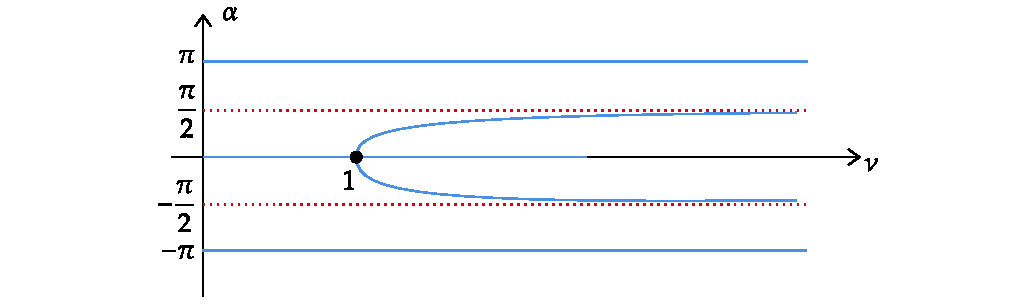
\includegraphics[scale=0.9]{figures/solutions/ch3/S01D01.pdf}
\end{figure}
The blue curves mark the location of the fixed points.


\item First we compute $\nabla f(x_1, x_2)$:
\begin{align}
	\nabla f(x_1, x_2) = \begin{pmatrix}
		0 & 1 \\
		\displaystyle \frac{g}{R}[2\nu \cos^2(x_1) - \cos(x_1) - \nu] & \displaystyle -\frac{b}{m}
	\end{pmatrix}
\end{align}
who's eigenvalues are given by
\begin{align}
	\lambda_\pm = -\frac{b}{2m} \pm \sqrt{\left(\frac{b}{2m}\right)^2 + \frac{g}{R}[2\nu \cos^2(x_1) - \cos(x_1) - \nu]}
\end{align}
Now we investigate the linear stability of each fixed point:

\textbf{Fixed point }$(0,0)$:
\begin{align}
	\lambda_\pm = -\frac{b}{2m} \pm \sqrt{\left(\frac{b}{2m}\right)^2 + \frac{g}{R}(\nu -1)}
\end{align}
\begin{itemize}
	\item $\nu < 1 \Longrightarrow$ Re$(\lambda_+)<0$ and Re$(\lambda_-)<0$. Therefore $(0,0)$ is asymptotically stable.
	
	\item $\nu > 1 \Longrightarrow$ Re$(\lambda_+)>0$ and Re$(\lambda_-)<0$. Therefore $(0,0)$ is unstable.
\end{itemize}

\textbf{Fixed points $(\pm \pi,0)$:}
\begin{align}
	\lambda_\pm = -\frac{b}{2m} \pm \sqrt{\left(\frac{b}{2m}\right)^2 + \frac{g}{R}(\nu + 1)}
\end{align}
For any $\nu \geq 0$, Re$(\lambda_+)>0 \Longrightarrow (\pm \pi,0)$ is unstable for any $\nu \geq 0$.


\textbf{Fixed points $(\pm \alpha_0,0)$}
Remember that these fixed points only exist when $\nu > 1$. Also $\cos(\pm \alpha_0) = \frac{1}{\nu}$
\begin{align}
	\lambda_\pm = -\frac{b}{2m} \pm \sqrt{\left(\frac{b}{2m}\right)^2 + \frac{g}{R}\left( \frac{1-\nu^2}{\nu} \right)}
\end{align}
For any $\nu > 1$, Re$(\lambda_+)<0$ and Re$(\lambda_-)<0$. Therefore the fixed points $(\pm \alpha_0,0)$ are asymptotically stable. 

\begin{figure}[h]
	\centering
	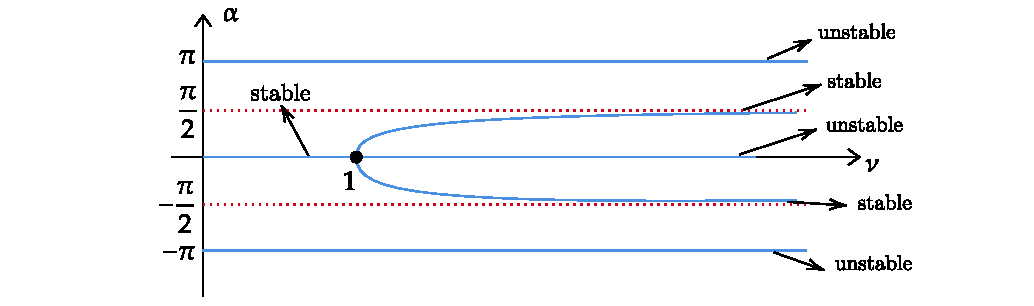
\includegraphics[scale=0.9]{figures/solutions/ch3/S01D02.pdf}
\end{figure}

The bifurcation of equilibria occurs at $\nu = 1 \Longrightarrow \Omega^2 = \frac{g}{R} \Longrightarrow \Omega = \pm \sqrt{\frac{g}{R}}$
\end{enumerate}
\end{solution}

\begin{solution}[3.3]
	\leavevmode
\begin{enumerate}
\item By setting $f(x)=0$, we obtain three fixed points for $\dot{x} = f(x)$. This can be seen by noting that the first equation $a(y_0 - x_0)=0$ implies $x_0 = y_0$. From the second equation, we get
\begin{align}
        &bx_0 - y_0 -x_0 z_0 = 0 \\
	&z_0 = b-1.
\end{align}

Then the third equation reduces to
\begin{align}
        &x_0y_0 - cz_0 = 0\\
        	&x_0=y_0 = \pm \sqrt{c(b-1)}.
\end{align}
The resulting three fixed points are
\begin{align}
	P_1 &: x_0 = y_0 = z_0 = 0\\
	P_2 &: x_0 = y_0 = \sqrt{c(b-1)} \;, z_0 = b-1 \\
	P_3 &: x_0 = y_0 = -\sqrt{c(b-1)} \;, z_0 = b-1.
\end{align}
For the system to have these three fixed points we must have $\boxed{b>1}$. If $0<b\leq1$, the only fixed point is $P_1$.

Let $A$ denote $Df(x_0,y_0,z_0)$. Then:
\begin{align}
	A = \begin{pmatrix}
		-a & a & 0 \\
		b-z_0 & -1 & -x_0 \\
		y_0 & x_0 & -c
	\end{pmatrix}
\end{align}

The eigenvalues $\lambda$ of $A$ are defined as the roots of the characteristic polynomial
$$
\det |A - \lambda I |=0.
$$
For the matrix $A$ this takes the form
\begin{align}
	A = \begin{vmatrix}
		-a-\lambda & a & 0 \\
		b-z_0 & -1-\lambda & -x_0 \\
		y_0 & x_0 & -c-\lambda
	\end{vmatrix} = 0.
\end{align}
We may expand this determinant according to the first row as

\begin{align}
&(-a-\lambda)\begin{vmatrix}-1-\lambda & -x_0 \\ x_0 & -c-\lambda \end{vmatrix} - a \begin{vmatrix} b-z_0 & -x_0 \\ y_0 & -c-\lambda \end{vmatrix} =0 \\
&-(a+\lambda)\left[ (1+\lambda) (c+\lambda) + x_0^2 \right] -a(b-z_0)(-c-\lambda) -ax_0y_0= 0
\end{align}
After collecting the coefficients of the different powers of $\lambda$, the characteristic equation of $A$ is:
\begin{align}
	\lambda^3 + (a+c+1)\lambda^2 + [ac + a + c + x_0^2 + a(z_0 - b)]\lambda + ac(z_0 - b + 1) + x_0^2a + ax_0y_0 = 0
\end{align}


\textbf{Stability of $P_1$:}
\begin{align}
	\lambda_3 + (a + c + 1)\lambda^2 + (ac + a + c -ab)\lambda - ac(b-1) = 0
\end{align}
A necessary condition for all roots of the above polynomial to be negative is that all its coefficients have the same sign. But here $-ac(b-1)<0$ while $\lambda^3$ has a positive coefficient (i.e. $+1$). $\Longrightarrow A$ has a positive eigenvalue.

$\Longrightarrow P_1$ is unstable.

\textbf{Stability of $P_2, P_3$:}
Note that in the characteristic equation, we only have products of $x_0$ and $y_0$, i. e. $x_0^2$ and $x_0y_0$. This means that the equation is invariant to changing the sign of $x_0$ and $y_0$ and we get the same eigenvalues at $P_2$ and at $P_3$. 

The Routh-Hurwitz determinants are:
\begin{align}
	d_1 &= 2ac(b - 1) > 0 \\
	d_2 &= (a + b)c > 0 \\
	d_3 &= \begin{vmatrix}
		(a + b)c & 2ac(b - 1) \\
		1 & a + c + 1
	\end{vmatrix} = (a + b)(a + c + 1)c - 2ac(b - 1)
\end{align}
For $P_2$ and $P_3$ to be unstable, we must have $d_3 < 0$
\begin{align}
	d_3 < 0 \Longleftrightarrow b > \frac{a(3 + a + c)}{a - (c + 1)} \underbrace{>}_{\text{follows from }a>c+1} 1
\end{align}

\item
\begin{verbatim}
	%% Initiate Script
	close all
	clear all
	clc
	
	%% Params & Initial Condition
	
	a = 10;
	b = 28;
	c = 8/3;
	
	x0 = [0.101; 0.1; 0.1];
	
	%% Function & Simulation
	
	f = @(t,x) [a * (x(2) - x(1));
	            b * x(1) - x(2) - x(1) * x(3);
	            x(1) * x(2) - c * x(3)];
	        
	[t ,x] = ode45(f, [0, 1000], x0);
	
	%% Plot
	
	figure(1)
	hold on
	plot3(x(:,1), x(:,2),x(:,3))
\end{verbatim}

\begin{figure}[h]
	\centering
	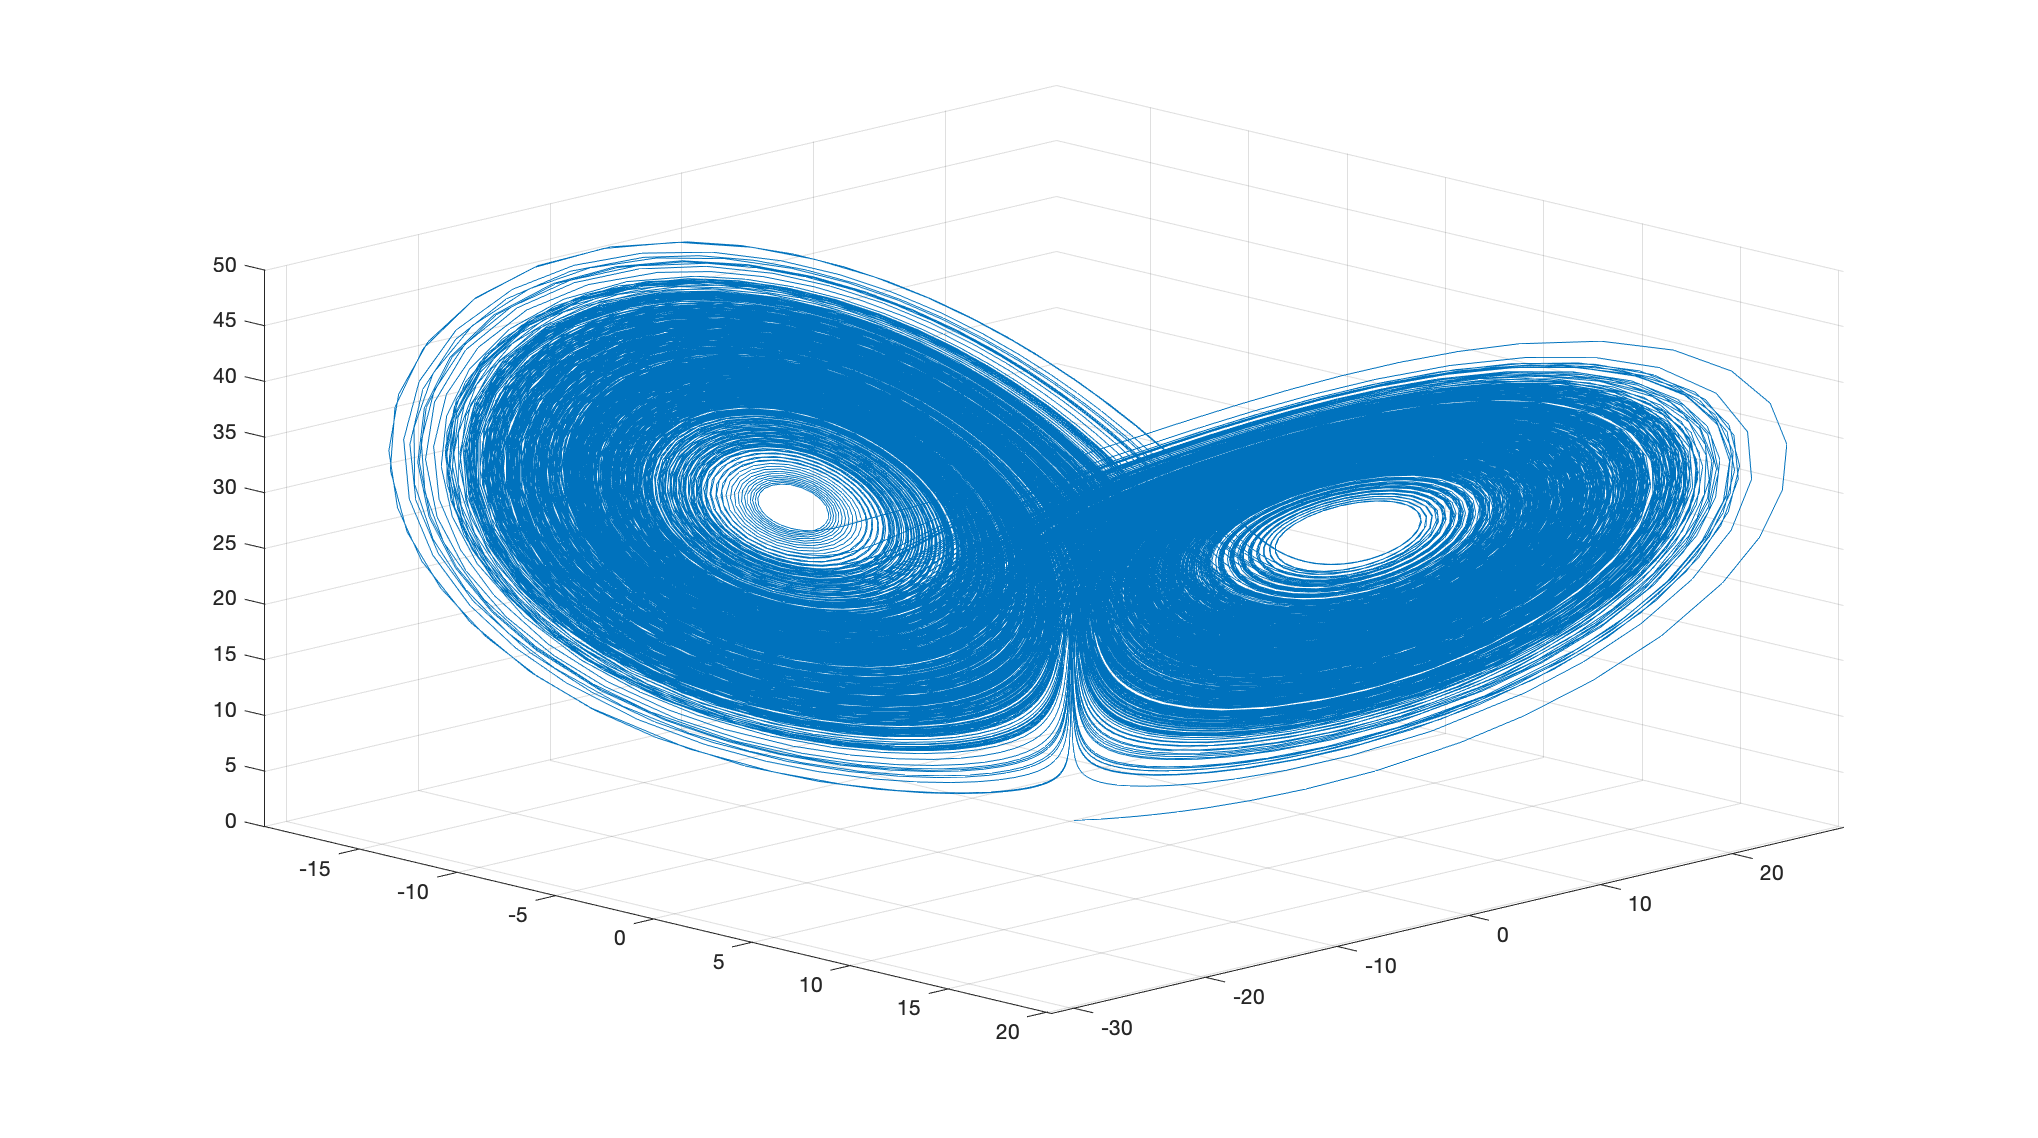
\includegraphics[scale=0.48]{figures/solutions/ch3/S03D01.pdf}
	\caption{Simulation of the Lorenz equations.}
\end{figure}
\end{enumerate}
\end{solution}

\begin{solution}[3.4]
	\leavevmode
\begin{align}
	E(x,\dot{x}) = \frac{1}{2}\dot{x}^2 + (1 - \cos(x))
\end{align}
\begin{align}
	y &= (y_1,y_2) := (x, \dot{x}) \\
	y &= f(y) = \begin{bmatrix}
		y_2 \\
		-cy_2 - \sin(y_1)
	\end{bmatrix} \Longrightarrow
	E(y) = \frac{1}{2}y_2^2 + (1 - \cos(y_1))
\end{align}

\begin{enumerate}
\item 
\begin{align}
	E(0) = 0, DE(0) = 0, D^2E(0) = \begin{bmatrix}
	1 & 0 \\ 0 & 1
	\end{bmatrix}
\end{align}
$\Longrightarrow$ Hessian is positive definite.

$\Longrightarrow E$ is positive-definite near the origin

\item 
\begin{align}
	\dot{E}(y) &= \langle DE(y),f(y) \rangle = (\sin(y_1),y_2) \cdot (y_2, -cy_2 - \sin(y_1)) \\
	&= \sin(y_1)y_2 - cy_2^2 -\sin(y_1)y_2 \\
	&= -cy_2^2 \leq 0
\end{align}
$E$ is positive definite around the origin and $\dot{E}$ is negative semi-definite.

Indeed, we cannot find an open set $U$ around the origin where
\begin{align}
	\dot{E}(y)<0 \;\; \forall y \in U\backslash \{0\} \;\; [\dot{E}(y)=0 \text{ for any } y = (y_1,0) \text{ with } y_1 \neq 0]
\end{align}
Thus, theorem 2 is not applicable to conclude nonlinear asymptotic stability of the origin.
\end{enumerate}
\end{solution}


\begin{solution}[3.5]
	\leavevmode
\begin{enumerate}
\item By setting $f(x)=0$, we obtain three fixed points for $\dot{x} = f(x)$. This can be seen by noting that the first equation $a(y_0 - x_0)=0$ implies $x_0 = y_0$. From the second equation, we get
\begin{align}
        &bx_0 - y_0 -x_0 z_0 = 0 \\
	&z_0 = b-1.
\end{align}

Then the third equation reduces to
\begin{align}
        &x_0y_0 - cz_0 = 0\\
        	&x_0=y_0 = \pm \sqrt{c(b-1)}.
\end{align}
The resulting three fixed points are
\begin{align}
	P_1 &:\ x_0 = y_0 = z_0 = 0\\
	P_2 &:\ x_0 = y_0 = \sqrt{c(b-1)} \;, z_0 = b-1 \\
	P_3 &:\ x_0 = y_0 = -\sqrt{c(b-1)} \;, z_0 = b-1.
\end{align}
For the system to have these three fixed points we must have $\boxed{b>1}$. If $0<b\leq1$, the only fixed point is $P_1$.

Let $A$ denote $Df(x_0,y_0,z_0)$. Then:
\begin{align}
	A = \begin{pmatrix}
		-a & a & 0 \\
		b-z_0 & -1 & -x_0 \\
		y_0 & x_0 & -c
	\end{pmatrix}
\end{align}

The eigenvalues $\lambda$ of $A$ are defined as the roots of the characteristic polynomial $\det |A - \lambda I |=0.$
For the matrix $A$ this takes the form
\begin{align}
	A = \begin{vmatrix}
		-a-\lambda & a & 0 \\
		b-z_0 & -1-\lambda & -x_0 \\
		y_0 & x_0 & -c-\lambda
	\end{vmatrix} = 0.
\end{align}
We may expand this determinant according to the first row as

\begin{align}
&(-a-\lambda)\begin{vmatrix}-1-\lambda & -x_0 \\ x_0 & -c-\lambda \end{vmatrix} - a \begin{vmatrix} b-z_0 & -x_0 \\ y_0 & -c-\lambda \end{vmatrix} =0 \\
&-(a+\lambda)\left[ (1+\lambda) (c+\lambda) + x_0^2 \right] -a(b-z_0)(-c-\lambda) -ax_0y_0= 0
\end{align}
After collecting the coefficients of the different powers of $\lambda$, the characteristic equation of $A$ is:
\begin{align}
	\lambda^3 + (a+c+1)\lambda^2 + [ac + a + c + x_0^2 + a(z_0 - b)]\lambda + ac(z_0 - b + 1) + x_0^2a + ax_0y_0 = 0
\end{align}


\textbf{Stability of $P_1$:}
\begin{align}
	\lambda_3 + (a + c + 1)\lambda^2 + (ac + a + c -ab)\lambda - ac(b-1) = 0
\end{align}
A necessary condition for all roots of the above polynomial to be negative is that all its coefficients have the same sign. But here $-ac(b-1)<0$ while $\lambda^3$ has a positive coefficient (i.e. $+1$). $\Longrightarrow A$ has a positive eigenvalue.

$\Longrightarrow P_1$ is unstable.

\textbf{Stability of $P_2, P_3$:}
Note that in the characteristic equation, we only have products of $x_0$ and $y_0$, i. e. $x_0^2$ and $x_0y_0$. This means that the equation is invariant to changing the sign of $x_0$ and $y_0$ and we get the same eigenvalues at $P_2$ and at $P_3$. 

The Routh-Hurwitz determinants are:
\begin{align}
	d_1 &= 2ac(b - 1) > 0 \\
	d_2 &= (a + b)c > 0 \\
	d_3 &= \begin{vmatrix}
		(a + b)c & 2ac(b - 1) \\
		1 & a + c + 1
	\end{vmatrix} = (a + b)(a + c + 1)c - 2ac(b - 1)
\end{align}
For $P_2$ and $P_3$ to be unstable, we must have $d_3 < 0$
\begin{align}
	d_3 < 0 \Longleftrightarrow b > \frac{a(3 + a + c)}{a - (c + 1)} \underbrace{>}_{\text{follows from }a>c+1} 1
\end{align}

\item
\begin{verbatim}[numbers = left]
	%% Initiate Script
	close all
	clear all
	clc
	
	%% Params & Initial Condition
	
	a = 10;
	b = 28;
	c = 8/3;
	
	x0 = [0.101; 0.1; 0.1];
	
	%% Function & Simulation
	
	f = @(t,x) [a * (x(2) - x(1));
	            b * x(1) - x(2) - x(1) * x(3);
	            x(1) * x(2) - c * x(3)];
	        
	[t ,x] = ode45(f, [0, 1000], x0);
	
	%% Plot
	
	figure(1)
	hold on
	plot3(x(:,1), x(:,2),x(:,3))
\end{verbatim}

\newpage

\begin{figure}[h]
	\centering
	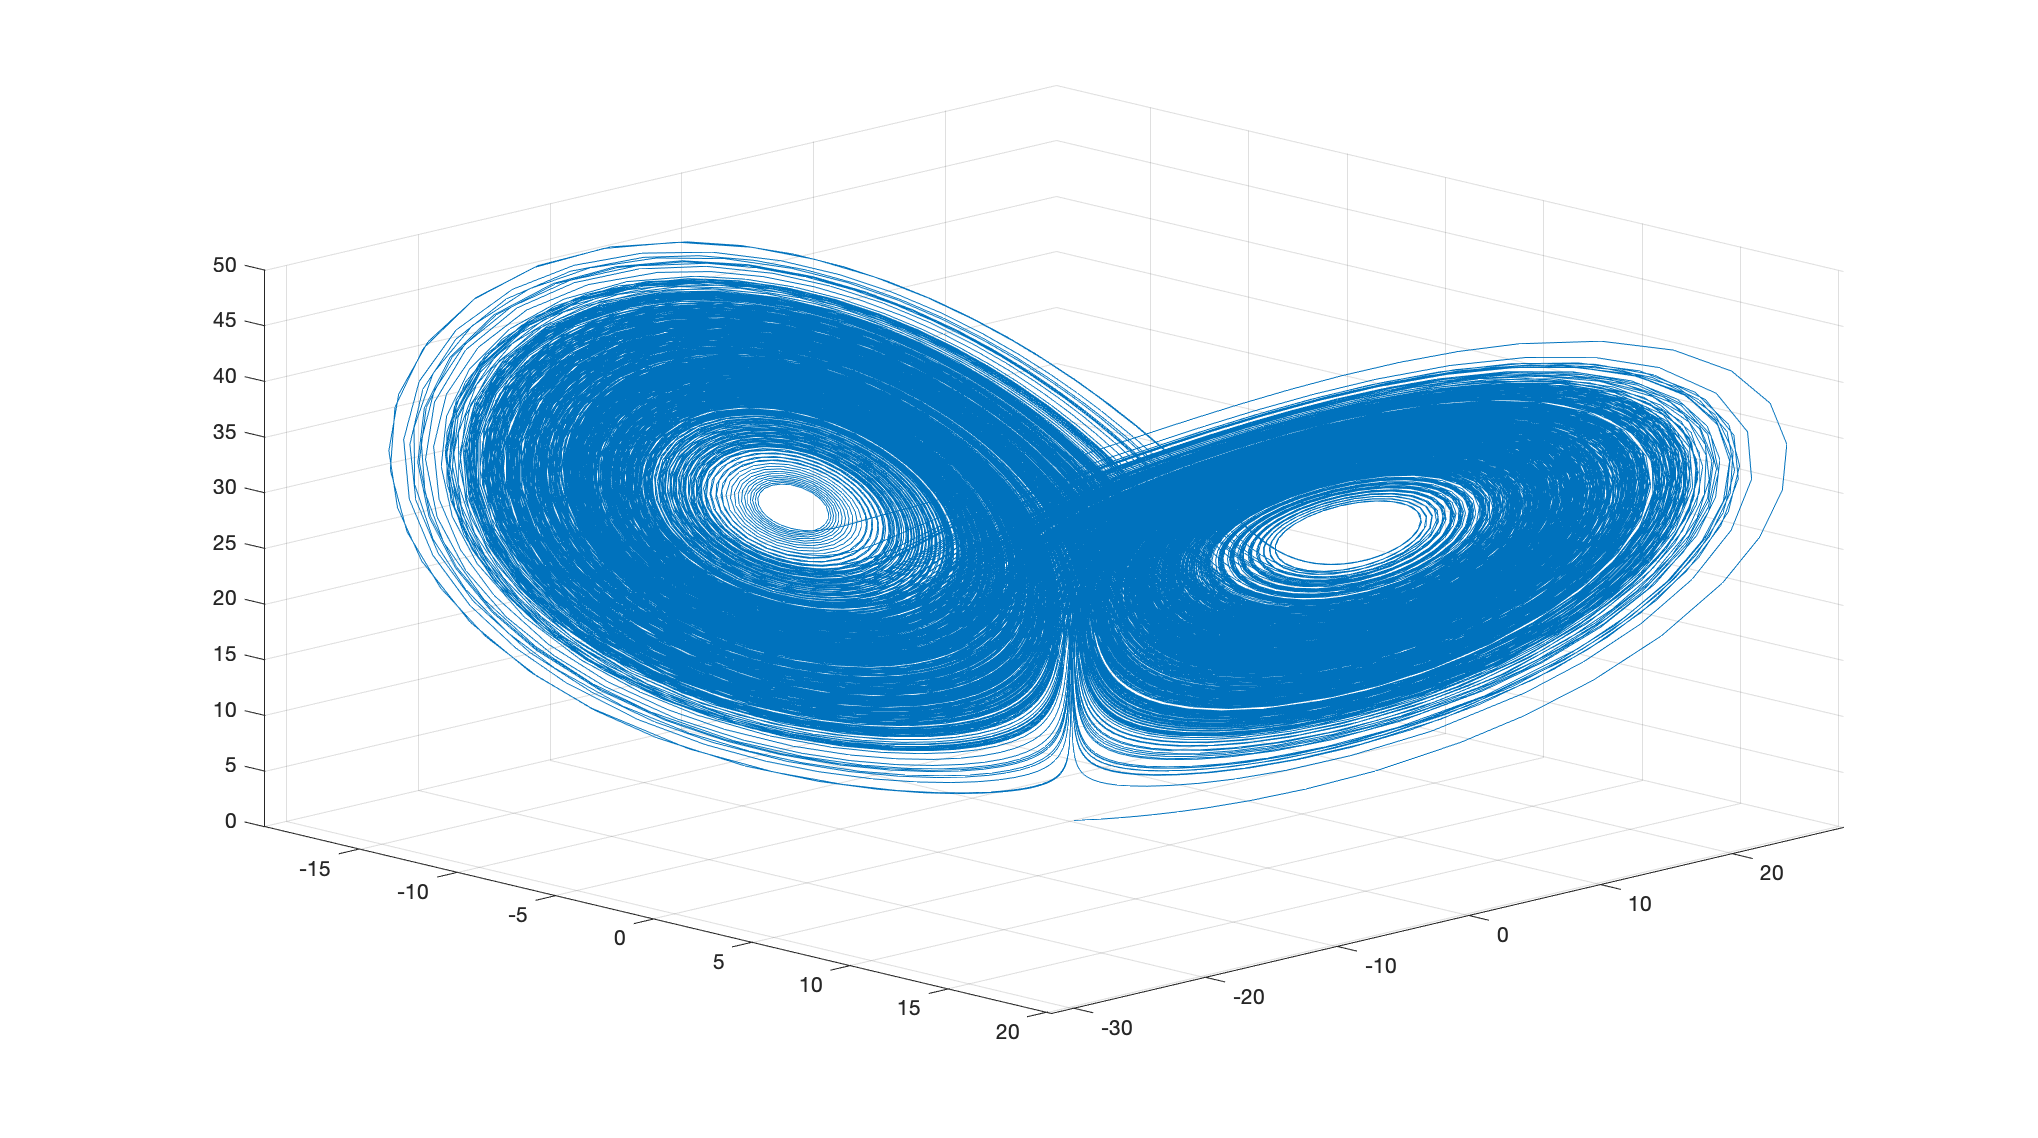
\includegraphics[scale=0.48]{figures/solutions/ch3/S03D01.pdf}
	\caption{Simulation of the Lorenz equations.}
\end{figure}
\end{enumerate}
\end{solution}


\begin{solution}[3.6]
We use Krasovski's theorem with $V = E, U \subset (-\pi, \pi) \times \mathbb{R}$ open set around the origin in $S' \times \mathbb{R}$ such that the statements (i) \& (ii) in the hypothesis of Krasovski are satisfied as shown above in part a).

\begin{align}
	S = \{ y \in U \vert \dot{E}(y)=0 \} \subset \underbrace{\{ (y_1, 0) \;\vert\; y_1 \in (-\pi,\pi) \}}_{\tilde{S}}
\end{align}
Indeed, the only trajectory of the system completely contained in the set $\tilde{S}$ on the $y_1$-axis is the origin (cf. phase portrait). $\Longrightarrow S$ contains only the fixed point as a trajectory of the system.

Hence, the hypothesis of Krasovski's theorem is satisfied and the origin is asymptotically stable for the nonlinear damped pendulum.
\end{solution}

\begin{solution}[3.7]
\begin{align}
	\dot{E}(y) &= \langle DE(y),f(y) \rangle = (\sin(y_1),y_2) \cdot (y_2, -cy_2 - \sin(y_1)) \\
	&= \sin(y_1)y_2 - cy_2^2 -\sin(y_1)y_2 \\
	&= -cy_2^2 \leq 0
\end{align}
$E$ is positive definite around the origin and $\dot{E}$ is negative semi-definite.

Indeed, we cannot find an open set $U$ around the origin where
\begin{align}
	\dot{E}(y)<0 \;\; \forall y \in U\backslash \{0\} \;\; [\dot{E}(y)=0 \text{ for any } y = (y_1,0) \text{ with } y_1 \neq 0]
\end{align}
Thus, theorem 2 is not applicable to conclude nonlinear asymptotic stability of the origin.
\end{solution}

\begin{solution}
First construct the function:
\begin{align}
	\bar{E}(q, \dot{q}) &= E(q, \dot{q}) - V(q_0) \\
	&= \frac{1}{2}\dot{q}^\text{T}M\dot{q} + V(q) - V(q_0)
\end{align}
Now, at $(q,\dot{q})=(q_0,0)$ we have $\bar{E}(q_0,0)=0$

Note that $M(q)$ is positive definite for all $q$ and $V(q) - V(q_0)$ is positive around $q=q_0$. (Since $V$ has a local minimum at $q_0$)

$\Longrightarrow \bar{E}(q,\dot{q})$ is positive definite around $(q_0,0)$.

But $\displaystyle \frac{d\bar{E}}{dt} = \frac{dE}{dt}$ since $V(q_0)$ is a constant.

We show that $\displaystyle \frac{dE}{dt}=0$.

First note that, in general, the Lagrangian equation of motion is a system of $n$ coupled equations with each equation given by:
\begin{align}
	\frac{d}{dt} \left[ \frac{\partial L}{\partial \dot{q}_k} \right] - \frac{\partial L}{\partial q_k} =0 \qquad k = 1,2,\ldots,n
\end{align}
Multiply each equation by $\dot{q}_k$ and sum over $k$ to get:

We'll use Einstein's notation: sum over repeated indices.

\begin{equation}\label{S03E041}
	\dot{q}_k \left[ \frac{d}{dt}\left( \frac{\partial L}{\partial \dot{q}_k} \right) - \frac{\partial L}{\partial q_k} \right] =0
\end{equation}
Since $\displaystyle L = \frac{1}{2}M_{ij}\dot{q}_i \dot{q}_j - V$ we have:

\begin{align}\label{S03E042}
		\frac{\partial L}{\partial \dot{q}_k} &= M_{ik}\dot{q}_i \quad , \quad \frac{\partial L}{\partial q_k} = \frac{1}{2} \frac{\partial M_{ij}}{\partial q_k}\dot{q}_i\dot{q}_j - \frac{\partial V}{\partial q_k} \\
		\frac{d}{dt} \frac{\partial L}{\partial \dot{q}_k} &= M_{ik}\ddot{q}_i + \frac{\partial M_{ik}}{\partial q_j}\dot{q}_j\dot{q}_i
\end{align}
Substituting (\ref{S03E042}) into (\ref{S03E041}), we get
\begin{align}
	M_{ik} \ddot{q}_i\dot{q}_k + \frac{\partial M_{ik}}{\partial q_j}\dot{q}_j\dot{q}_i\dot{q}_k - \frac{1}{2}\frac{\partial M_{ij}}{\partial q_k}\dot{q}_i\dot{q}_j\dot{q}_k + \frac{\partial V}{\partial q_k}\dot{q}_k = 0
\end{align}
Since there is a sum over repeated indices we have:
\begin{align}
	M_{ik}\ddot{q}_i\dot{q}_k &\equiv M_{ij}\ddot{q}_i\dot{q}_j & \frac{\partial M_{ik}}{\partial q_j}\dot{q}_j\dot{q}_i\dot{q}_k &\equiv \frac{\partial M_{ij}}{\partial q_k}\dot{q}_i\dot{q}_j\dot{q}_k
\end{align}
\begin{align}
	\Longrightarrow \underbrace{M_{ij}\ddot{q}_i\dot{q}_j + \frac{1}{2} \frac{\partial M_{ij}}{\partial q_k}\dot{q}_i\dot{q}_j\dot{q}_k + \frac{\partial V}{\partial q_k}\dot{q}_k}_{ \displaystyle =\frac{d}{dt}\left[ \frac{1}{2}M_{ij}\dot{q}_i\dot{q}_j+V(q) \right]} = 0
\end{align}
\begin{align}
	\Longrightarrow \left[ \frac{1}{2}\dot{q}^\text{T}M(q)\dot{q} + V(q) \right] = 0 \Longrightarrow \frac{dE}{dt}=0 \Longrightarrow \frac{d\bar{E}}{dt}=0
\end{align}
Using $\bar{E}$ as the Lyapunov function, we conclude that $(q_0,0)$ is a \underline{stable} equilibrium point.
\end{solution}


\begin{solution}[4.1]
\begin{enumerate}
\item Let the graph of the center manifold near the origin be given by $y = h(x), \; h:\mathbb{R}^c \rightarrow \mathbb{R}^d$
\begin{figure}[h]
	\centering
	
\includegraphics[scale=0.9]{figures/solutions/ch4/S01D01.pdf}
\end{figure}
By the invariance of the center manifold we have $y_n = h(x_n)$ for all $n$.

\begin{align}
	y_{n+1} = h(x_{n+1})
\end{align}
But
\begin{align}
	y_{n+1} &= By_n + g(x_n, y_n) \\
	&= Bh(x_n) + g(x_n, h(x_n))
\end{align}
and
\begin{align}
	x_{n+1} &= Ax_n + f(x_n, y_n) \\
	&= Ax_n + f(x_n, h(x_n))
\end{align}
Hence
\begin{align}
	Bh(x_n) + g(x_n, h(x_n)) = h[Ax_n + f(x_n, h(x_n))]
\end{align}
Therefore, the function $h:\mathbb{R}^c \rightarrow \mathbb{R}^d$ satisfies

\begin{align}\label{S04E011}\boxed{
		Bh(x) + g(x, h(x)) = h[Ax + f(x, h(x))]
	}
\end{align}


\item Here, $[A] = [1],\; [B] = [\lambda], \; f(x_n,y_n) = x_ny_n$ and $g(x_n, y_n)=-x_n^2$.

Since $h$ passes through the origin and it is tangent to the $x$-axis, we have $h(0)=0$ and $h'(0)=0$. (Note that here $c=d=1 \Rightarrow h:\mathbb{R} \rightarrow \mathbb{R}$).

Therefore, the Taylor expansion of $h$ around $x=0$ has the form
\begin{align}\label{S04E012}
	h(x) = ax^2 + bx^3 + \mathcal{O}(x^4)
\end{align}
Equation (\ref{S04E011}) for the current system is: $\lambda h(x) - x^2 = h(x + xh(x))$.

Substituting (\ref{S04E012}) in this equation we get
\begin{align}
	\lambda(ax^2 + bx^3 + \mathcal{O}(x^4)) - x^2 &= h[x + ax^3 + \mathcal{O}(x^4)] \\
	&= a(x + ax^3 + \mathcal{O}(x^4))^2 + b(x + ax^3 + \mathcal{O}(x^4))^3 + \cdots
\end{align}
\begin{align}
	\Longrightarrow (\lambda a - 1)x^2 + \lambda b x^3 + \mathcal{O}(x^4) = ax^2 + bx^3 + \mathcal{O}(x^4)
\end{align}
Matching the exponents from both sides we obtain:
\begin{align}
	\lambda a - 1 = a &\Longrightarrow a = \frac{1}{\lambda - 1} \\
	\lambda b = b &\Longrightarrow b = 0
\end{align}
and finally
\begin{align}
	\boxed{
		h(x) = \frac{1}{\lambda - 1}x^2 + \mathcal{O}(x^4)	
	}
\end{align}


\item The center manifold near the origin satisfies $h(x) \approx \frac{1}{\lambda - 1}x^2$.
Hence, the dynamics on the center manifold satisfy

\begin{align}
	x_{n+1} &= x_n + \frac{1}{\lambda - 1}x_n^3 \nonumber \\
	\Longrightarrow x_{n+1} &= x_n \left( 1 + \frac{1}{\lambda - 1}x_n^2 \right) \label{S04E013}
\end{align}
In the following, we show that the fixed point $x=0$ of (\ref{S04E013}) is asymptotically stable. 

First let $x_0 \in \mathbb{R}$ with $|x_0|>0$ small enough be an initial condition. Then if
\begin{align}\label{S04E014}
	\left\vert 1 + \frac{1}{\lambda - 1}x_0^2 \right\vert < 1
\end{align}
we have
\begin{align}
	|x_1| \leq \left\vert x_0 \left( 1 + \frac{1}{\lambda - 1}x_0^2 \right) \right\vert < |x_0|
\end{align}
Inequality (\ref{S04E014}) holds if and only if $|x_1| < |x_0| < \sqrt{2(1-\lambda)}$. That is for any $x_0$ with $|x_0|<\sqrt{2(1-\lambda)}$ we have $|x_1| < |x_0| < \sqrt{2(1-\lambda)}$.

For such initial conditions, we have (by induction):
\begin{align}\label{S04E015}
	\cdots < |x_{n+1}| < |x_n| < \cdots < |x_1| < |x_0| < \sqrt{2(1-\lambda)}
\end{align}
This proves that the stability of the fixed point $x=0$. To prove asymptotic stability, we need
\begin{align}
	\lim_{n \rightarrow \infty} x_n = 0
\end{align}

Note that the sequence $\{|x_n|\}$ is a decreasing (due to (\ref{S04E015})) sequence that is bounded from below $(|x_n| \geq 0)$. Therefore, it must have a limit:
\begin{align}
	\lim_{n \rightarrow \infty} |x_n| = \alpha
\end{align}

This limit, in general, doesn't have to be zero. But taking the limit $n \rightarrow \infty$ in equation (\ref{S04E013}) we get
\begin{align}
	\lim_{n \rightarrow \infty} |x_{n+1}| = \lim_{n \rightarrow \infty}
	|x_n| \left( 1 + \frac{1}{\lambda - 1} \lim_{n \rightarrow \infty} |x_n|^2 \right)
\end{align}
\begin{align}
	\alpha = \alpha \left( 1 + \frac{1}{\lambda - 1} \alpha^2 \right) \Longrightarrow \alpha = 0 \Longrightarrow \lim_{n \rightarrow \infty} x_n = 0
\end{align}
Therefore the fixed point is asymptotically stable.
\vspace{15 pt}
The following figure shows the iterations of the map for four initial conditions marked by square symbols. The higher iterations are marked by dots. The black curve marks the approximate center manifold:
\begin{align}
	y = \frac{1}{\lambda - 1}x^2
\end{align}


\begin{verbatim}
	%% Initiation

	close all
	clear all
	clc

	%% Main

	lambda = 0.5;
	x = linspace(-0.5, 0.5, 50);
	
	y = x.^2/(lambda - 1);
	
	figure;
	plot(x,y)
	
	maxIter = 1000;
	
	xn = zeros(maxIter + 1, 1);
	yn = zeros(maxIter + 1, 1);
	
	% Initial Conditions
	
	xn1(1) = -0.1;
	yn1(1) = 0.1;
	
	xn2(1) = 0.1;
	yn2(1) = 0.1;
	
	xn3(1) = -0.25;
	yn3(1) = 0.25;
	
	xn4(1) = 0.25;
	yn4(1) = 0.25;
	
	% Interations
	
	for j = 1:maxIter
	    [xn1(j+1), yn1(j+1)] = map(xn1(j), yn1(j), lambda);
	end
	
	for j = 1:maxIter
	    [xn2(j+1), yn2(j+1)] = map(xn2(j), yn2(j), lambda);
	end
	
	for j = 1:maxIter
	    [xn3(j+1), yn3(j+1)] = map(xn3(j), yn3(j), lambda);
	end
	
	for j = 1:maxIter
	    [xn4(j+1), yn4(j+1)] = map(xn4(j), yn4(j), lambda);
	end
	
	hold on
	plot(xn1, yn1, '*r')
	plot(xn2, yn2, '*r')
	plot(xn3, yn3, '*g')
	plot(xn4, yn4, '*g')
	xlabel('$x$','interpreter','latex')
	ylabel('$y$','interpreter','latex')
	grid on
		
	%% Function
	
	function [x1, y1] = map(x0, y0, lambda)
	    x1 = x0 + x0 * y0;
	    y1 = lambda * y0 - x0^2;
	end
\end{verbatim}

This MATLAB code gives the following figure:
\begin{figure}[h]
	\centering
	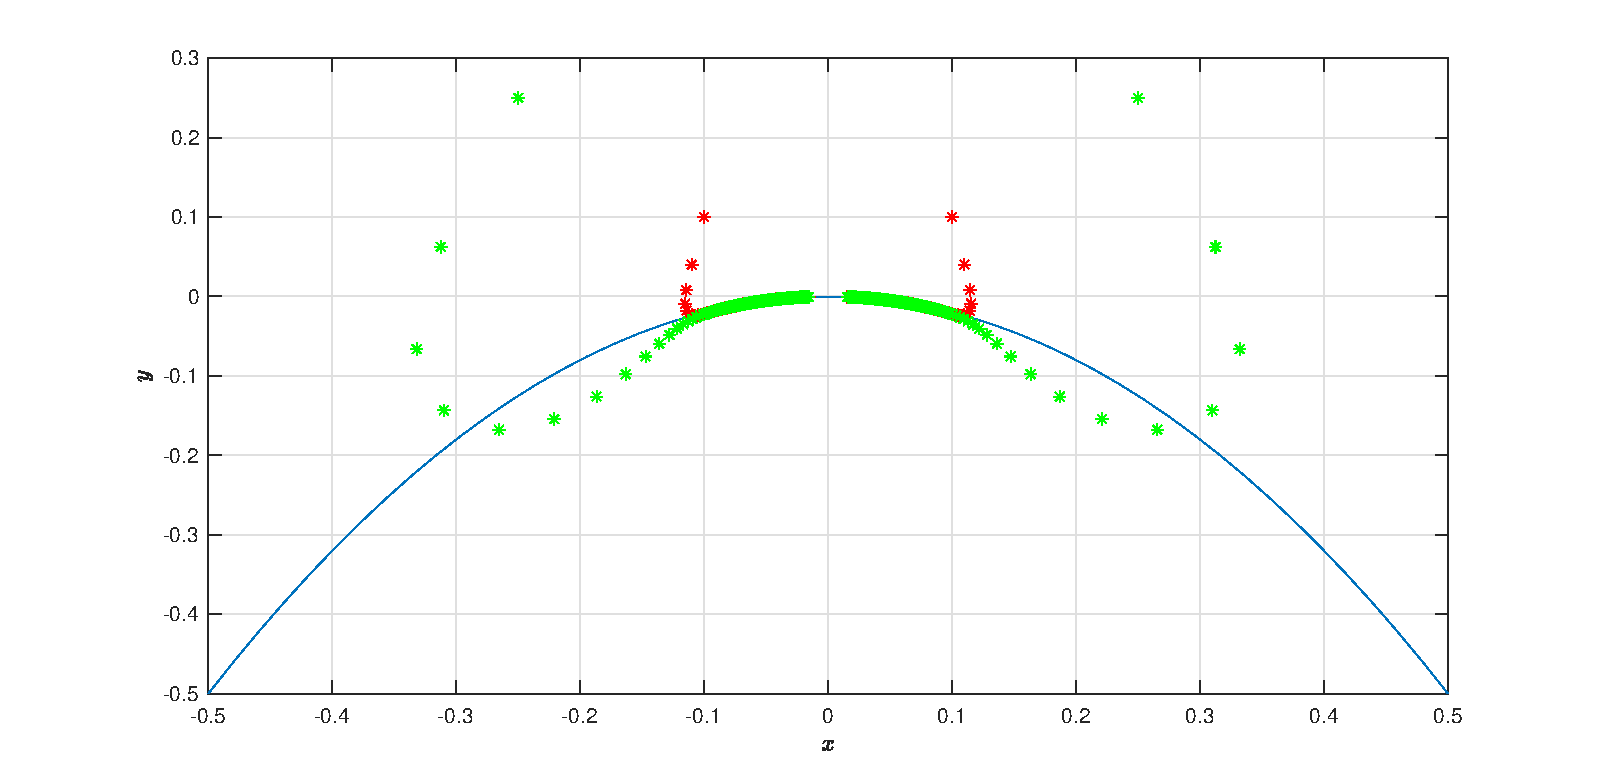
\includegraphics[scale=0.5]{figures/solutions/ch4/S01D02.pdf}
\end{figure}
\end{enumerate}
\end{solution}


\begin{solution}[4.2]
\begin{figure}[h]
	\centering
	\includegraphics[scale=0.9]{figures/solutions/ch4/S02D01.pdf}
\end{figure}
Let $x_1 = x$ and $x_2 = \dot{x}$. Then:
\begin{align}
	\begin{dcases}
		\dot{x}_1 = x_2 \\
		\dot{x}_2 = -\sin(x_1)
	\end{dcases}
\end{align}
By linearization, one can show that the fixed point $(\pi, 0)$ is an unstable hyperbolic fixed point with stable and unstable linear subspaces spanned by $\begin{pmatrix} 1 \\ 1 \end{pmatrix}$ and $\begin{pmatrix} 1 \\ -1 \end{pmatrix}$, respectively:
\begin{figure}[h]
	\centering
	
\includegraphics[scale=0.9]{figures/solutions/ch4/S02D02.pdf}
\end{figure}
For convenience, we shift the origin by the transformation $\xi_1 = x_1 - \pi$ and $\xi_2 = x_2$ such that in $(\xi_1 , \xi_2)$ the origin is the hyperbolic fixed point.

In this coordinate system, the dynamical system becomes:
\begin{align}
	\begin{dcases}
		\dot{\xi}_1 = \xi_2 \\
		\dot{\xi}_2 = \sin(\xi_1)
	\end{dcases} \qquad (\text{since } -\sin(x_1) = -\sin(\xi_1 + \pi) = \sin(\xi_1))
\end{align}
The unstable manifold passing through the origin is a graph over $\xi_1$ and tangent to $E^U$.
\begin{figure}[h]
	\centering
	
\includegraphics[scale=0.9]{figures/solutions/ch4/S02D03.pdf}
\end{figure}
If this graph is given by $\xi_2 = h(\xi_1)$, the Taylor expansion of $h$ looks like:
\begin{align}
	h(\xi_1) = \underbrace{0}_{h(0)=0} + \underbrace{\xi_1}_{h'(0)=1} + a\xi_1^2 + b\xi_1^3 + \mathcal{O}(\xi_1^4)
\end{align}
By invariance of the unstable manifold we have $\dot{\xi}_2 = h'(\xi_1) \dot{\xi}_1$

Therefore,
\begin{align}
	\sin(\xi_1) = (1 + 2a\xi_1 + 3b\xi_1^2 + \mathcal{O}(3))(\xi_1 + a\xi_1^2 + b\xi_1^3 + \mathcal{O}(4))
\end{align}
The Taylor expansion of $\sin(\xi_1)$ around $\xi_1=0$ reads
\begin{align}
	\sin(\xi_1) = \xi_1 - \frac{1}{6}\xi_1^3 + \mathcal{O}(\xi_1^5)
\end{align}
Matching exponents we get $a = 0$ and $b = -\frac{1}{24}$.

Therefore, the graph of unstable manifold satisfies:
\begin{align}
	\xi_2 = \xi_1 - \frac{1}{24}\xi_1^3 + \mathcal{O}(\xi_1^4)
\end{align}
or
\begin{align}\boxed{
	x_2 = x_1 - \pi -\frac{1}{24}(x_1 - \pi)^3 + \mathcal{O}(|x_1 - \pi|^4)
}\end{align}
\end{solution}

\begin{solution}[4.3]
	\leavevmode
\begin{enumerate}
\item Linearized dynamics around fixed point $(0,0)$
\begin{align}
	\dot{\eta} = A\eta \; , \; A = \begin{bmatrix}
		0 & 1 \\ \beta & -\delta
	\end{bmatrix} \; , \; \text{eig}(A) = \lambda_{1,2} = -\delta \pm \sqrt{\delta^2 - \beta}
\end{align}
Note that $\lambda_1 = 0 \; , \; \lambda_2 = -\delta$ for $\beta = 0$. Thus, by the center manifold theorem, we have a 1-dimensional center manifold passing through the origin and a unique 1-dimensional stable manifold.

Consider the extended system
\begin{align}
	\dot{\beta} &= 0 \\
	\begin{bmatrix}
		\dot{u} \\ \dot{v}
	\end{bmatrix}
	&= \underbrace{\begin{bmatrix}
		0 & 1 \\ 0 & -\delta
	\end{bmatrix}}_{B} \begin{bmatrix}
		u \\ v
	\end{bmatrix}
	+
	\begin{bmatrix}
		0 \\ \beta u - u^2
	\end{bmatrix}
\end{align}

\begin{align}
	& \text{Eigenvalues of } B: \lambda_1 = 0 \; , \; \lambda_2 = -\delta \\
	& \text{Eigenvectors of } B: e_1 = \begin{bmatrix}
		1 \\ 0
	\end{bmatrix} \; , \; e_2 = \begin{bmatrix}
		\frac{1}{\delta} \\ -1
	\end{bmatrix}
\end{align}
From the eigenvalues and eigenvectors, we can perform a change of coordinates
\begin{align}
	\begin{bmatrix}
		u \\ v
	\end{bmatrix} = T \begin{bmatrix}
		x \\ y
	\end{bmatrix} \; , \; T = [e_1 \vert e_2] = \begin{bmatrix}
		1 & \frac{1}{\delta} \\ 0 & -1
	\end{bmatrix} \; , \; T^{-1} = \begin{bmatrix}
		1 & \frac{1}{\delta} \\ 0 & -1
	\end{bmatrix} = T
\end{align}
\begin{align}
	\Longrightarrow u = x + \frac{y}{\delta} \; , \; v = -y
\end{align}

\begin{align}
	\Longrightarrow \begin{bmatrix}
		\dot{x} \\ \dot{y}
	\end{bmatrix} &= T^{-1}BT \begin{bmatrix}
		x \\ y
	\end{bmatrix} + T^{-1} \begin{bmatrix}
		0 \\ \beta u - u^2
	\end{bmatrix} \nonumber \\
	\label{S04E021}
	&= \begin{bmatrix}
		0  & 0 \\ 0 & -\delta
	\end{bmatrix} \begin{bmatrix}
		x \\ y
	\end{bmatrix} + \begin{bmatrix}
		\frac{1}{\delta} \left( \beta \left( x + \frac{y}{\delta} \right) - \left( x + \frac{y}{\delta} \right)^2 \right) \\
		-\beta \left( x + \frac{y}{\delta} \right) + \left( x + \frac{y}{\delta} \right)^2
	\end{bmatrix} 
\end{align}

Seek center manifold as a graph over center subspace locally as

\begin{align}
	y &= h(x, \beta) = a_1x^2 + a_2x\beta + \underbrace{a_3\beta^2}_{=0} + \mathcal{O}(3) \nonumber \\
	\label{S04E022}
	\dot{y} &= \frac{\partial h}{\partial x}\dot{x} + \frac{\partial h}{\partial \beta} \underbrace{\dot{\beta}}_{0}
\end{align}
Note: We cancel the term $a_3 \beta^2$ to respect the existence of the fixed point.

Use invariance in (\eqref{S04E022}): 
\begin{align}
	\label{S04E023}	
	\Longrightarrow \dot{y} &= (2a_1x + a_2 \beta) \left[ \frac{1}{\delta} \left( \beta \left( x + \frac{h(x,\beta)}{\delta} \right) - \left( x + \frac{h(x,\beta)}{\delta} \right)^2 \right) \right] \\
	\label{S04E024}	
	\text{But also } \dot{y} &= -\delta h(x, \beta) - \beta \left( x + \frac{h(x,\beta)}{\delta} \right) + \left( x + \frac{h(x, \beta)}{\delta} \right)^2
\end{align}
Comparing $\mathcal{O}(2)$ terms in (\ref{S04E023}) \& (\ref{S04E024}), we get:
\begin{align}
	x^2: \qquad -\delta a_1 + 1 = 0 &\Longrightarrow a_1 = \frac{1}{\delta} \\
	x\beta: \qquad -\delta a_2 - 1 = 0 &\Longrightarrow -a_2 = \frac{1}{\delta}
\end{align}
Thus, the $\beta$-dependent center manifold is given by
\begin{equation} \label{S04E025}
	h(x, \beta) = \frac{x^2}{\delta} - \frac{x \beta}{\delta} + \mathcal{O}(3)
\end{equation} 
Substitute (\ref{S04E025}) into first equation in (\ref{S04E021}) to obtain reduced dynamics on the center manifold: $W^C_\beta (0)$ up to quadratic order.
\begin{align}
	\dot{x} &= \frac{1}{\delta} \left[ \beta \left( x + \frac{h(x, \beta)}{\delta} \right) - \left( x + \frac{h(x, \beta)}{\delta} \right)^2 \right] \\
	&= \frac{1}{\delta} [\beta x - x^2] + \mathcal{O}(3)
\end{align}

\item 
\begin{align}
	\dot{x} = \frac{1}{\delta} [\beta x - x^2]
\end{align}
Fixed points:
\begin{align}
	x &= 0, \\
	\beta &= x
\end{align}

\begin{figure}[h]
	\centering
	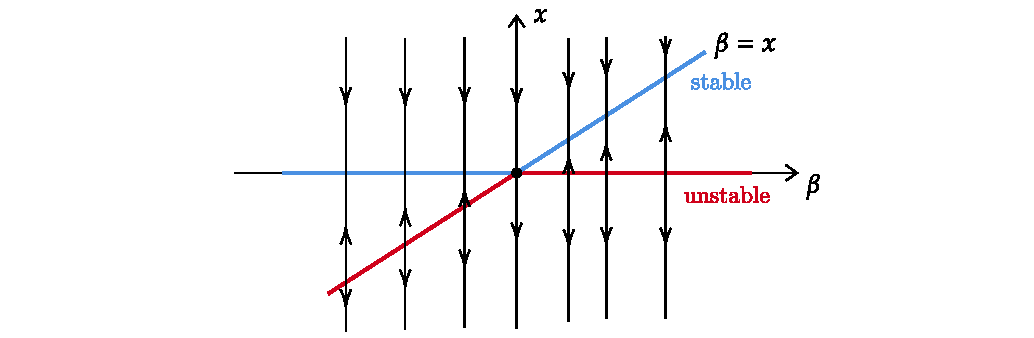
\includegraphics[scale=0.9]{figures/solutions/ch4/S05D01.pdf}
	\caption{Transcritical bifurcation}
\end{figure}
\end{enumerate}
\end{solution}

\begin{solution}[4.4]
\begin{enumerate}
	\item Let $x_1=x$ and $x_2=\dot{x}$. Then the system can be written as
\begin{align}
	\begin{dcases}
\dot{x}_1&=x_2\\
\dot{x}_2&=-\frac{k}{m}x_1 -\frac{c}{m}x_2 +\frac{1}{m}F_f(x_2).
	\end{dcases}
\end{align}

The fixed point is at 
\begin{align}
x^{0}_1=\frac{1}{k}F_f(0)=\frac{mg\mu_0}{k}\left(1+e^{-\beta|v_0|} \right)\text{sign }(v_0), \quad x^{0}_2=0.
\end{align}

Let us now shift the origin to the fixed point by introducing new coordinates as $z_1 = x_1 - x^0_1$ and $z_2=x_2$. 
Then 
\begin{align}
\label{eq111}
\dot{z}_1&=z_2\\
\dot{z}_2&=-\frac{k}{m}z_1 -\frac{c}{m}z_2 +\frac{1}{m}F_f(z_2)-\frac{1}{m}F_f(0),
\end{align}
with the fixed point at $z_1=z_2=0$. The linearized system is given by
\begin{align}
\dot{\xi}=\begin{pmatrix} 0 & 1 \\ -\frac{k}{m} & \mu \end{pmatrix}\xi, 
\end{align}
where we have introduced the parameter
\begin{align}
\boxed{\mu=\frac{1}{m}\left(F_f'(0)-c\right) = g\beta \mu_0 e^{-\beta|v_0|}-\frac{c}{m}}. 
\end{align}
The eigenvalues of the coefficient matrix are 

\begin{align}
\label{eq12}
\lambda_{1,2} = \frac{\mu}{2}\pm \frac{1}{2}\sqrt{\mu^2-\frac{4k}{m}}.
\end{align}
For the remainder of the discussion, let us assume that  $|\mu|$ is not too big; specifically $\mu^2 < \frac{4k}{m}$. This is in line with our previous assumption to treat $\mu$ as a bifurcation parameter. In this case, the real part of $\lambda_{1,2}$ can simply be read off from \eqref{eq12} as 

\begin{align}
\text{Re }(\lambda_{1,2}) = \frac{\mu}{2}. 
\end{align}

As a result, if $\mu<0$ then Re $(\lambda_1)<0$ and Re $(\lambda_2)<0$, hence the fixed point is \underline{asymptotically stable} by the Hartman-Grobman theorem. This condition translates into
\begin{align}
\mu<0 \Leftrightarrow g\beta\mu_0e^{-\beta|v_0|}<\frac{c}{m} \Leftrightarrow |v_0| > \frac{1}{\beta}\log\left(\frac{mg\beta \mu_0}{c} \right).
\end{align}

Hence, if 
\begin{align}
\label{eqcond}
|v_0| > \frac{1}{\beta}\log\left(\frac{mg\beta \mu_0}{c} \right),
\end{align}
then $(z_1=z_2=0)$ is an asymptotically stable fixed point. 

\begin{remark}[]
Note that if the viscous damping $c$ is large enough such that $c>mg\beta \mu_0$ then $\log\left(\frac{mg\beta \mu_0}{c} \right)<0$. Then the condition \eqref{eqcond} is satisfied for any $v_0\neq 0$ and ($z_1=z_2=0$) is asymptotically stable for any $v_0$.
\end{remark}

\item For $0<\mu \ll 1$ we have Re $(\lambda_{1,2})>0$. At $\mu=0$ the eigenvalues cross the imaginary axis at 
	\begin{align}
\lambda_{1,2}(\mu=0)=\pm i \sqrt{\frac{4k}{m}}.
	\end{align}
Now let $-1\ll\mu< 0$. Then the eigenvalues are 
\begin{align}
\lambda_{1,2}=\frac{\mu}{2}\pm i\frac{1}{2} \sqrt{\frac{4k}{m}-\mu^2}.
\end{align}

Define 
\begin{align}
\label{eq14}
\boxed{\delta(\mu)=\frac{\mu}{2}, \quad \omega(\mu)=\frac{1}{2}\sqrt{\frac{4k}{m}-\mu^2}.}
\end{align}
Then, we can separate the linear and nonlinear terms from the system \eqref{eq111} and write it as
\begin{align}
\label{transf}
\begin{pmatrix} \dot{z}_1 \\ \dot{z}_2 \end{pmatrix} = A\begin{pmatrix} z_1 \\ z_2 \end{pmatrix} + \begin{pmatrix} 0 \\ \frac{1}{m}F_f(z_2)-\frac{1}{m}F'_f(0)z_2 - \frac{1}{m}F_f(0)\end{pmatrix},
\end{align}
where we have denoted the linear part as $$A=\begin{pmatrix} 0 & 1 \\ -\frac{k}{m} & \mu \end{pmatrix}.$$ The eigenvalues of $A$ are $\delta(\mu)\pm i \omega(\mu)$. To simplify the calculation of the eigenvectors, we note that  (as a consequence of \eqref{eq14})

\begin{align}
\mu = 2\delta \quad \frac{k}{m} = \delta^2 + \mu^2
\end{align}
and hence
\begin{align}
A=\begin{pmatrix}0 & 1 \\ -\delta^2 -\omega^2 & 2\delta  \end{pmatrix}.
\end{align}

We then search for a vector $s$ such that 

\begin{align}
As-(\delta + i\omega)s =\begin{pmatrix}-\delta - i\omega & 1 \\ -\delta^2 -\omega^2 & \delta-i\omega  \end{pmatrix}   \begin{pmatrix} s_1 \\ s_2\end{pmatrix}.
\end{align}

For example, the non-normalized vector

\begin{align}
s = \begin{pmatrix} 1  \\ \delta + i\omega \end{pmatrix}
\end{align}

is a good choice. To separate the real and imaginary parts of the eigenvector we write it as 
\begin{align}
s= \begin{pmatrix} 1\\ \delta(\mu) \end{pmatrix}\pm i \begin{pmatrix} 0 \\ \omega(\mu) \end{pmatrix}.
\end{align}

Selecting the real and imaginary parts of $s$ as basis vectors then puts $A$ in the desired block-diagonal form,  that is 
\begin{align}
A=VDV^{-1},
\end{align}

where 
\begin{align}
D=\begin{pmatrix} \delta & \omega \\ -\omega & \delta \end{pmatrix} \text{ and } V=\begin{pmatrix} 1 & 0 \\ \delta & \omega  \end{pmatrix}.
\end{align}

This means, that under  the change of variables 
\begin{align}
\begin{pmatrix} z_1 \\ z_2 \end{pmatrix} = V \begin{pmatrix} u \\ v\end{pmatrix}
\end{align}
 we get the transformed dynamical system
 
 \begin{align}
 \begin{pmatrix} \dot{u} \\ \dot{v} \end{pmatrix} = \begin{pmatrix} \delta  & \omega  \\  -\omega & \delta \end{pmatrix}\begin{pmatrix} u \\ v  \end{pmatrix} + \frac{1}{m\omega}\begin{pmatrix} 0  \\ F_f(\delta u + \omega v) - F'_f(0)(\delta u + \omega v) - F_f (0)\end{pmatrix}.
 \end{align}
 This is the desired form for the dynamical system defined in the problem description. Note that we may put
 \begin{align}
 f(x,y,\mu) &=0 \\
 g(x,y,\mu) &= \frac{1}{m\omega} F_f(\delta u + \omega v) - F'_f(0)(\delta u + \omega v) - F_f (0)
 \end{align}
 to compute the desired parameters
 
 \begin{align}
d_0 = \delta'(0)=\frac{1}{2}, \quad \omega_0 = \omega(0)= \sqrt{\frac{k}{m}}, \quad a_0 = \frac{kg\mu_0 \beta^3 e^{-\beta |v_0|}}{16m},
 \end{align}
where we have used that 
\begin{align}
g_{vvv}(0,0,0) = \frac{k}{m^2}F'''(0)= \frac{kg\mu_0 \beta^3 e^{-\beta |v_0|}}{m}.
\end{align}

According to the Hopf-Bogdanov theorem, the radial component of the normal form of the dynamics can be written as
\begin{align}
\boxed{\dot{r}=r\left( \frac{\mu}{2}+ \frac{kg\mu_0 \beta^3 e^{-\beta |v_0|}}{16m}r^2\right)},
\end{align}
which has fixed points 
\begin{align}
	r&=0 \text{ which corresponds to the stable fixed point} \\
	r &= \pm \sqrt{\frac{-8\mu m e^{\beta |v_0|}}{kg\mu_0 \beta^3}}, \text{ which corresponds to the unstable limit cycle. }
\end{align}

Expressed as a function of $v_0$, the bifurcation occurs at 
\begin{align}
v_C = \frac{1}{\beta}\log \left(\frac{mg\beta \mu_0}{c} \right).
\end{align}

\item For $\mu<0$ the amplitude of the unstable limit cycle is 

\begin{align}
r_0 = \sqrt{\frac{-8\mu m e^{\beta |v_0|}}{kg\mu_0 \beta^3}}
\end{align}
\end{enumerate}
\end{solution}

\begin{solution}[5.1]
Consider a planar dynamical system with the following phase portrait:

\begin{figure}[h]
	\centering
	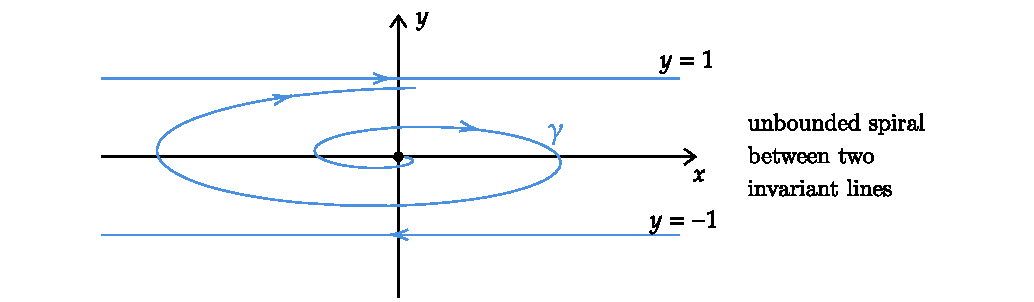
\includegraphics[scale=0.9]{figures/solutions/ch5/Q04D01.pdf}
	\caption{Phase portrait of the planar dynamical system}
\end{figure}

Which of the following statement is true?

\begin{enumerate}
	\item The $\omega$-limit set of $\gamma$ is empty.
	\item By the Poincaré-Bendixson theorem, the $\omega$-limit set of $\gamma$ is composed of the lines $y = 1$ and $y = -1$.
	\item \underline{The Poincaré-Bendixson theorem does not apply to $\gamma$.}
	\item None of the above
\end{enumerate}
\end{solution}

\begin{solution}[5.2]
\begin{align}
	\begin{bmatrix}\label{S05E011}
		\dot{x} \\
		\dot{y}
	\end{bmatrix} =
	\underline{F}(x,y) := \begin{bmatrix}
		\displaystyle \frac{\partial H}{\partial y}(x,y) + f_1(x,y) \\
		\displaystyle -\frac{\partial H}{\partial x}(x,y) + f_2(x,y)
	\end{bmatrix}
\end{align}
\begin{align}
	\text{div}(\underline{F}) &= \frac{\partial^2 H}{\partial x \partial y}(x,y) + \frac{\partial f_1}{\partial x}(x,y) - \frac{\partial^2 H}{\partial y \partial x}(x,y) + \frac{\partial f_2}{\partial y} \\
	&= \text{div}(\underline{f}) \qquad (H \in C^2) \\
	&\neq 0 \quad \forall (x,y)\in \mathbb{R}^2
\end{align}
Thus, by the Bendixson's criterion, \eqref{S05E011} does not have a periodic solution in $\mathbb{R}^2$.
\end{solution}


\begin{solution}[6.1]
Remember from the lecture on averaging that $\dot{x} = \varepsilon f(x,t, \varepsilon)$ can be transformed to the differential equation
\begin{align}\label{S05E021}
	\dot{\tilde{x}} = \varepsilon \bar{f}_0(\tilde{x}) + \varepsilon^2f_1(\tilde{x},t,\varepsilon)
\end{align}
Through the near-identity transformation $x = \tilde{x} + \varepsilon w(\tilde{x},t)$.

Moreover, $f_1$ is globally bounded, i.e., there exists $L_1 > 0$ such that
\begin{align}
	|f_1(\tilde{x},t,\varepsilon)| < L_1 \qquad \forall t > 0 \text{ and } \forall \tilde{x}\in \mathbb{R}^n
\end{align}
Now by construction $|x(t) - \tilde{x}(t)| = \varepsilon|w(\tilde{x}(t),t)| = \mathcal{O}(\varepsilon)$
Therefore, it suffices to show that solutions of the averaged equation
\begin{align}\label{S05E022}
	\dot{y} = \varepsilon \bar{f}_0(y)
\end{align}
remain $\mathcal{O}(\varepsilon)$ close to the solutions of (\ref{S05E021}).

Subtracting \eqref{S05E022} from \eqref{S05E021}, integrating and dropping the tilde (\textasciitilde) sign, we get 
\begin{align}
	x(t) - y(t) = x_0 - y_0 + \varepsilon \int_0^t \left( \bar{f}_0(x(s)) - \bar{f}_0(y(s)) \right) \, \text{d}s + \varepsilon^2 \int_0^t f_1(x(s),s,\varepsilon) \, \text{d}s
\end{align}
\begin{align}
	\Longrightarrow |x(t) - y(t)| \leq |x_0 - y_0| + \varepsilon \int_0^t L_2|x(s) - y(s)|\,\text{d}s + \varepsilon^2 \int_0^t L_1 \,\text{d}s
\end{align}
where we used boundedness of $f_1$ and Lipschitz continuity of $\bar{f}_0$:
\begin{align}
	|f_0(x) - f_0(y)| \leq L_2 |x - y|
\end{align}
Therefore,
\begin{align}\label{S05E023}
	|x(t) - y(t)| \leq |x_0 - y_0| + \varepsilon^2 L_1t + \int_0^t \varepsilon L_2 |x(s) - y(s)|\,\text{d}s
\end{align}
Now apply Gronwall's inequality with $v(t) = |x(t) - y(t)|$, $u(t) = \varepsilon L_2$ and $c(t) = |x_0 - y_0| + \varepsilon^2 L_1t$ to get
\begin{align}
	|x(t) - y(t)| &\leq |x_0 - y_0|e^{\varepsilon L_2 t} + \int_0^t \varepsilon L_1 e^{\varepsilon L_2 (t-s)}\,\text{d}s \\
	&= |x_0 - y_0|e^{\varepsilon L_2 t} + \varepsilon \frac{L_1}{L_2} \left( e^{\varepsilon L_2 t} -1 \right) \leq \left[ |x_0 - y_0| + \varepsilon \frac{L_1}{L_2} \right] e^{\varepsilon L_2 t}
\end{align}
Since $|x_0 - y_0| = \mathcal{O}(\varepsilon)$, we conclude that $|x(t) - y(t)|= \mathcal{O}(\varepsilon)$ as long as $t\in \left[0,\frac{1}{\varepsilon L_2}\right)$, i.e., time scales of $\mathcal{O}(1/\varepsilon)$.
\end{solution}


\begin{solution}[6.2]
We start with the Taylor expansions of $u(x,y,t)$ and $v(x,y,t)$ in $y$ near $y=0$:
\begin{align}\label{S05E031}
	\begin{cases}
		\displaystyle u(x,y,t) = u(x,0,t) + \frac{\partial u}{\partial y}(x,0,t)y + \mathcal{O}(|y|^2) \\
		\displaystyle v(x,y,t) = v(x,0,t) + \frac{\partial v}{\partial y}(x,0,t)y + \frac{1}{2} \frac{\partial^2 v}{\partial y^2}(x,0,t)y^2 + \mathcal{O}(|y|^3)
	\end{cases}
\end{align}
But $u(x,0,t) = v(x,0,t) = 0$ for any $x$.

Differentiating $u(x,0,t) = 0$ with respect to $x$ we get $\displaystyle \frac{\partial u}{\partial x}(x,0,t) = 0$. By incompressibility we have
\begin{align}
	\frac{\partial u}{\partial x} &= - \frac{\partial v}{\partial y} \\
	\Longrightarrow \frac{\partial v}{\partial y}(x,0,t) &= - \frac{\partial u}{\partial x}(x,0,t) = 0, \;\; \forall x
\end{align}
Hence \eqref{S05E031} simplifies to
\begin{align}
	\begin{cases}
		\displaystyle u(x,y,t) = \frac{\partial u}{\partial y}(x,0,t)y + \mathcal{O}(|y|^2) = y U(x,y,t) \\
		\displaystyle v(x,y,t) = \frac{1}{2} \frac{\partial^2 v}{\partial y^2}(x,0,t)y^2 + \mathcal{O}(|y|^3) = y^2V(x,y,t)
	\end{cases}
\end{align}
Also note that
\begin{align}\label{S05E032}
	\begin{cases}
		\displaystyle U(x,y,t) = \frac{\partial u}{\partial y}(x,0,t) \\
		\displaystyle V(x,y,t) = \frac{1}{2}\frac{\partial^2 v}{\partial y^2}(x,0,t)
	\end{cases}
\end{align}
Higher-order terms are identically zero. Therefore,
\begin{align}
	\begin{cases}
		\dot{x} = yU(x,y,t) \\
		\dot{y} = y^2V(x,y,t)
	\end{cases}
\end{align}
Scaling $y$ as $y = \varepsilon \eta$, we get:
\begin{align}\label{S05E033}
	\begin{cases}
		\dot{x} = \varepsilon \eta U(x,\varepsilon \eta, t) \\
		\dot{\eta} = \varepsilon \eta^2 V(x, \varepsilon \eta,t)
	\end{cases}
\end{align}
Since $U$ and $V$ are also $T$-periodic, averaging theory applies to \eqref{S05E033} with the averaged equations
\begin{align}\label{S05E034}
	\begin{cases}
		\dot{x} = \varepsilon \eta \bar{U}(x) \\
		\dot{\eta} = \varepsilon \eta^2 \bar{V}(x)
	\end{cases}
\end{align}
where
\begin{align}\label{S05E035}
	\begin{cases}
		\displaystyle \bar{U}(x) = \frac{1}{T} \int_0^T U(x,0,s)\,\text{d}s = \frac{1}{T} \int_0^T \frac{\partial u}{\partial y}(x,0,s)\,\text{d}s \\
		\displaystyle \bar{V}(x) = \frac{1}{T} \int_0^T V(x,0,s)\,\text{d}s = \frac{1}{2T} \int_0^T \frac{\partial^2 v}{\partial y^2}(x,0,s)\,\text{d}s
	\end{cases}
\end{align}

Rescaling time as $\displaystyle \frac{d\tau}{dt}=\eta(t)$ and denoting the derivative with respect to $\tau$ by prime sign ($'$) we get
\begin{align}
	\dot{x} = \frac{dx}{dt} = \frac{dx}{d\tau}\frac{d\tau}{dt} = \eta x' \quad , \quad \dot{\eta}= \eta \eta'
\end{align}

Substituting these expressions in \eqref{S05E035}, we get
\begin{align}\label{S05E036}
	\begin{cases}
		x' = \varepsilon \bar{U}(x) \\
		\eta' = \varepsilon \eta \bar{V}(x)
	\end{cases}
\end{align}

Equation \eqref{S05E036} has a fixed point $(x_0, \eta=0)$ on the wall if and only if $\bar{U}(x_0,0)=0$. Using \eqref{S05E035}, we have
\begin{align}\label{S05E037}
	\bar{U}(x_0) = 0 \Longleftrightarrow \boxed{\int_0^T \frac{\partial u}{\partial y}(x_0,0,s)\,\text{d}s = 0}
\end{align}

Now we turn to the stability of the fixed point $(x_0,0)$ on the wall by linearising \eqref{S05E036} around this fixed point:
\begin{align}
	\underline{\xi}' = \varepsilon \underbrace{\begin{pmatrix}
		\displaystyle \frac{\partial \bar{U}}{\partial x}(x_0) & 0 \\
		0 & \displaystyle \bar{V}(x_0)
	\end{pmatrix}}_{:=A} \underline{\xi}
\end{align}
The matrix $A$ has eigenvalues $\displaystyle \varepsilon \frac{\partial \bar{U}}{\partial x}(x_0)$ and $\varepsilon \bar{V}(x_0)$ corresponding to eigenvectors $\displaystyle \begin{pmatrix} 1 \\ 0 \end{pmatrix}$ and $\displaystyle \begin{pmatrix} 0 \\ 1 \end{pmatrix}$ respectively.

For the unstable manifold to be off the wall, we need $\bar{V}(x_0)>0$. Using \eqref{S05E035}, we have
\begin{align}\label{S05E038}
	\bar{V}(x_0) > 0 \Longleftrightarrow \boxed{\int_0^T \frac{\partial^2 v}{\partial y^2}(x_0,0,s)\,\text{d}s > 0}
\end{align}
\end{solution}

